\documentclass[11pt,oneside]{article}    %use"amsart"insteadof"article"forAMSLaTeXformat
\usepackage{geometry}        %Seegeometry.pdftolearnthelayoutoptions.Therearelots.
\geometry{letterpaper}        %...ora4paperora5paperor...
%\geometry{landscape}        %Activateforforrotatedpagegeometry
%\usepackage[parfill]{parskip}        %Activatetobeginparagraphswithanemptylineratherthananindent
\usepackage{graphicx}                %Usepdf,png,jpg,orepswithpdflatex;useepsinDVImode
                                %TeXwillautomaticallyconverteps-->pdfinpdflatex        
\usepackage{amssymb}
\usepackage[colorlinks]{hyperref}

%----macros begin---------------------------------------------------------------
\usepackage{color}
\usepackage{amsthm}

\def\conv{\mbox{\textrm{conv}\,}}
\def\aff{\mbox{\textrm{aff}\,}}
\def\E{\mathbb{E}}
\def\R{\mathbb{R}}
\def\Z{\mathbb{Z}}
\def\tex{\TeX}
\def\latex{\LaTeX}
\def\v#1{{\bf #1}}
\def\p#1{{\bf #1}}
\def\T#1{{\bf #1}}

\def\vet#1{{\left(\begin{array}{cccccccccccccccccccc}#1\end{array}\right)}}
\def\mat#1{{\left(\begin{array}{cccccccccccccccccccc}#1\end{array}\right)}}

\def\lin{\mbox{\rm lin}\,}
\def\aff{\mbox{\rm aff}\,}
\def\pos{\mbox{\rm pos}\,}
\def\cone{\mbox{\rm cone}\,}
\def\conv{\mbox{\rm conv}\,}
\newcommand{\homog}[0]{\mbox{\rm homog}\,}
\newcommand{\relint}[0]{\mbox{\rm relint}\,}

%----macros end-----------------------------------------------------------------

\title{LAR-ABC, a representation of architectural geometry \\
{\Large From concept of spaces, to design of building fabric, to construction simulation}
\footnote{This document is part of the \emph{Linear Algebraic Representation with CoChains} (LAR-CC) framework~\cite{cclar-proj:2013:00}. \today}
}
\author{Alberto Paoluzzi \and Enrico Marino \and Federico Spini}
%\date{}                            %Activatetodisplayagivendateornodate

\begin{document}
\maketitle
%\nonstopmode

\begin{abstract}
This paper discusses the application of LAR (Linear Algebraic Representation) scheme~\cite{Dicarlo:2014:TNL:2543138.2543294} to the whole architectural design process, from initial concept of spaces, to the additive manufacturing of design models, to the meshing for CAE analysis, to the detailed design of components of building fabric, to the BIM processing of quantities and costs. LAR (see, e.g. [1]) is a novel general and simple representation scheme for geometric design of curves, surfaces and solids, using simple, general and well founded concepts from algebraic topology. 
LAR supports all topological incidence structures, including enumerative (images), decompositive (meshes) and boundary (CAD) representations. It is dimension-independent, and not restricted to regular complexes. Furthermore, LAR enjoys a neat mathematical format, being based on chains, the domains of discrete integration, and cochains, the discrete prototype of differential forms, so naturally integrating the geometric shape with the supported physical properties. 
The LAR representation find his roots in the design language Plasm~\cite{Paoluzzi2003a}, and is currently embedded in python and javascript, providing the designer with powerful and simple tools for a geometric calculus of shapes. In this paper we introduce the motivation of this approach, discussing how it compares to other mixed-dimensionality representations of geometry and is supported by open-source software projects. We also discuss simple examples of use, with reference to various stages of the design process.
\end{abstract}

\newpage
\tableofcontents
\newpage

%-------------------------------------------------------------------------------
%===============================================================================
\section{Introduction}\label{sec:intro}
%===============================================================================
%-------------------------------------------------------------------------------
Looking for simplicity. 
Form and function. Who comes first?
CAD is evolving with the net.
Algebraic topology on graphics processors.

In this paper we discuss a novel linear algebraic representation, supporting topological methods to represent and process mesh connectivity information for dimension-independent cellular complexes, including simplicial, cuboidal, and polytopal cells. This representation works even with the awkward domain partitions---with non-convex and/or non-manifold cells, and cells non homeomorphic to balls---that may arise in Building Information Modeling (BIM) and Geographic Information Systems (GIS) applications. Simplicial and cuboidal cell complexes provide the standard mesh representation used in most science and engineering simulations, whereas complexes of possibly non-convex or non-contractible cells may be needed to represent the built environment in software applications for the Architecture, Engineering, and Construction (AEC) sector.

Our approach provides a unified representation where concepts and techniques from computer graphics (graphics primitives), geometric modelling (curves and surfaces) and solid modelling (solids and higher dim manifolds) converge with those from computational science (structured and unstructured meshes) in a common computational structure. This representation may be used in novel and highly demanding application areas\footnote{It is being tested within the \href{http://standards.ieee.org/develop/project/3333.2.html}{IEEE P3333.2} -- Standard for Three-Dimensional Model Creation Using Unprocessed 3D Medical Data.} (see for instance Figure~\ref{fig:bone}), and may be supported by modern silicon-based APIs\footnote{A prototype implementation with  \href{http://www.khronos.org/opencl/}{OpenCL} and \href{http://www.khronos.org/webcl/}{WebCL} is on the way.} on last and next generation hardware.


%-------------------------------------------------------------------------------
%===============================================================================
\section{Linear Algebraic Representation}\label{sec:lar}
%===============================================================================
%-------------------------------------------------------------------------------
\subsection{Representation scheme}
%-------------------------------------------------------------------------------
% 1 column
A foundational concept. Mapping from mathematical models to computer representations. 
Taxonomy: decompositive, enumerative, boundary, procedural representations.
The de-facto standard of PLM systems: non-manifold data structures + NURBS. 
Old, expensive, and inflexible.
Towards big geometric data. The need for rethinking the foundations. 
Algebraic geometry is here to stay. Sparse matrices and GPGPU.

%-------------------------------------------------------------------------------
\subsection{Topological operations}
%-------------------------------------------------------------------------------
% 1 column
Space decompositions. Chains as subsets of spaces. Cochains as fields over chains. Geometric integration: pairing of chains and cochains. Homology and cohomology. Boundary and coboundary operators. A single SpMV multiplication to compute the boundary of any chain of spaces.
Transposition and coboundary. Coboundary and operators of vector analysis: gradient, curl, divergenze, and Laplacian. Integration of geometry and physics through topological structures. Topological queries. The $d$-star of every cell. Decomposition of big structures and distributed computing.

%-------------------------------------------------------------------------------
\subsection{Models and structures}
%-------------------------------------------------------------------------------
% 2 columns
Model = Topology + Geometry. Model as embedded topology. Topology as the list of higher-dimensional cells of a space decomposition. The classical representation of cells via the list of their vertices. Composition of linear operators as the product of their matrices.
Fast transposition and product operations via GPGPU and OpenCL. Structures as hierarchical aggregation of space-instanced models and/or other structures. The representation of structures as ordered sequences of strictres, models and operators. Data Base of structures. The traversal of structures at run-time.

%===============================================================================
\section{LAR for Architecture, Building and Construction}\label{sec:abc}
%===============================================================================
%-------------------------------------------------------------------------------
\subsection{Architectural structures: the organisation of spaces}
%-------------------------------------------------------------------------------
% 1 column
Organic or rational architecture? Form from function or vice-versa? In either case, space units produce organised assemblies of spaces with more or less specialised functions. In set-theoretical terms, they provide either a partitioning or a covering of the building space. At the very end, an architectural design defines a topology of the space, as a collection of subsets (of space), closed with respect to finite intersection and union. 

In practical terms, the design concept will result in a cellular decomposition of the space, where elementary space units, either open or closed or partially open, establish pairwise adjacency relations; even before of any concrete embedding, i.e. even before that a global shape is envisioned by the architect. 

In the majority of cases, the geometric embedding of the design topology will produce a partitioning of space with plane or curved surfaces, and some horizontal or vertical composition of use patterns. In common building and construction, most of the separating surfaces will be either horizontal or vertical, but different arrangements of space cells are possible.

LAR-ABC requires that the topology is first defined hierarchically, producing finally a space plan subdivided by layers, where the junctions of at least three separating surfaces are identified and numbered. The simplest data definition is, of course, via the production of planar architectural drawings embedded in a common reference system.

%-------------------------------------------------------------------------------
\subsection{Models, structures, assemblies}
%-------------------------------------------------------------------------------

In LAR-ABC we make a distinction between geometric \emph{models}, \emph{structures}, and \emph{assemblies}. Some terminology and definitions are given below.

\paragraph{Geometric model}
A geometric \emph{model} is a pair (\emph{geometry},\emph{topology}) in a given coordinate system, where  \emph{topology} is the LAR specification of highest dimensional cells of a cellular decomposition of the model space, and \emph{geometry} is specified by the coordinates of \emph{vertices}, the spatial embedding of 0-cells of the cellular decomposition of space. From a coding viewpoint, a model is either an instance of the \texttt{Model} class, or simply a pair (\texttt{vertices}, \texttt{cells}), where \texttt{vertices} is a two-dimensional array of floats arranged by rows, and where the number of columns (i.e.~of \emph{coordinates}) equals the dimension $n$ of the embedding Euclidean space $\E^n$. Similarly, \texttt{cells} is a list of lists of vertex indices, where every list of indices corresponds to one of $d$-dimensional \emph{cells} of the space partition, with $d\leq n$.

\paragraph{Structure}
A \emph{structure} is the LAR representation of a hierarchical organisation of spaces into substructures, that may be organised into lower-level substructures, and so on, where each part \emph{may} be  specified in a \emph{local coordinate system}. Therefore, a structure is given as an \emph{(ordered) list of substructures and transformations} of coordinates, that apply to all the substructures following in the same list. A structure actually represents a \emph{graph of the scene}, since a substructure may be given a name, and referenced more than one time within one or more other structures.  The \emph{structure network}, including references, can be seen as an acyclic directed multigraph. In coding term, a structure is an instance of the \emph{Struct} class, whose parameter is a list of either other structures, or models, or transformations of coordinates, or references to structures or models.

\paragraph{Assembly}
An assembly is an \emph{(unordered) list of models} all \emph{embedded in the same coordinate space}, i.e.~all using the same coordinate system (the \emph{world coordinate system}). A assembly may be either defined by the user as a list of models, or automatically generated by the \emph{traversal} of a structure network. At traversal time, all the traversed structures and models are transformed from their local coordinate system to the world coordinates, that correspond to the coordinate frame of the root of the traversed network, i.e.~to the first model of the structure passed as argument to the \texttt{evalStruct} function, that implements the traversal algorithm. In few words, we can say that an assembly is the linearised version of the traversed structure network, where all the models are using the world coordinate system.

%===============================================================================
\section{The design of LAR-ABC}
%===============================================================================

LAR-ABC is a python library for geometric design of building objects with the Linear Algebraic Representation (LAR) specialised for Architecture, Building and Construction (ABC). In the present first prototype implementation of the library, we concentrate on the first two letters of this specification, namely the organisation of spaces (architecture) and the specification of physical, concrete components (building). 

%-------------------------------------------------------------------------------
\subsection{Concept design and project plan}
%-------------------------------------------------------------------------------
The client needs and wishes are initially specified by some initial set of requirements, traduced by the architect firm into a design concept, better specified by an initial project plan.
When the project plan is accepted by the client, giving a definite shape to the first architectural concept, the model of construction is usually a 2.5D model, made by opaque or transparent 2D surfaces embedded in 3D space. 

In this stage, LAR-ABC allows for the computation of every topological or geometrical property of interest, including the evaluation of the surface of the building envelope and its partitioning into subsets with different thermal requirements, as well as the computation of the internal volume, and its partitioning into any classes of internal space, and will grant any other geometric computation or simulation (for example of the thermal behaviour) of possible interest for the architect or the client.

%-------------------------------------------------------------------------------
\subsection{Building objects: components and assemblies}
%-------------------------------------------------------------------------------

The LAR description of the topology and its geometric embedding, defined by the position vectors of vertices or control points of the surfaces, makes possible to (mostly) automatically generate a first 3D model of the physical construction, i.e.~of the concrete instances of building components.

This (semi-)automatic transformation from a 2.5D model formed by surfaces to a 3D model formed by assemblies of solid objects, is obtained using the boundary operator, that allow to discriminate between the various subsystems of the building fabric, i.e.~between the horizontal and vertical enclosures, the horizontal and vertical partitions of the interior, the elements of horizontal and vertical communications, and so on, as we show in Section~\ref{sec:examples}. 


\subsubsection{Some operators for assemblies}
%-------------------------------------------------------------------------------
Remember that an assembly is a \emph{list} of geometric models, i.e.is a list of pairs made by vertices and cells. Therefore, few specialised higher-level functions are needed to apply the typical operations of models to assemblies. Some higher-order general utilities for handling geometric assemblies are given below.  



\paragraph{Some operators for assemblies}
The function \texttt{larCells} is used to apply a given \texttt{fun} to the \emph{cells} of every LAR model contained in \texttt{assembly}. Conversely, \texttt{larVerts} is used to apply a given \texttt{fun} to the \emph{vertices} of every model in the \texttt{assembly}. Also, \texttt{larBinOps} allows to apply a binary \texttt{op}aeration to every argument pair generated by right distribution of the \texttt{arg} argument over the models contained in \texttt{assembly}.

%-------------------------------------------------------------------------------
@D Some operators for assemblies
@{
def larCells(fun):
    def larCells0(assembly):
        return TRANS(CONS([S1,COMP([AA(fun),S2])])(TRANS(assembly)))
    return larCells0

def larVerts(fun):
    def larCells0(assembly):
        return TRANS(CONS([ COMP([AA(fun),S1]),S2 ])(TRANS(assembly)))
    return larCells0

def larBinOps(op):
    def larCells0(assembly):
        def larCells1(arg):
            return AA(op)(DISTR([assembly,arg]))
        return larCells1
    return larCells0
@}
%-------------------------------------------------------------------------------

\paragraph{Low-dimensional constructors: 1D and 0D}
The \texttt{larQuote1D} function replicates the behaviour of the PLaSM \texttt{QUOTE} operator, where \texttt{pattern} is a list of either positive or negative numbers, respectively used to fill solid or empty intervals on the real line, producing as output a 1D LAR model. The \texttt{larQuote0D} function is used to embed several instances of a $d$-dimensional model in $\E^d$, i.e.~to compte a Cartesian product of models without increasing neither the embedding nor the intrinsic dimensions. A typical case use is to compute the $d$-skeleton (needed for the $\partial_{d+1}$ operator) in a $(d+1)$-dimesional extrausion.

%-------------------------------------------------------------------------------
@D Low-dimensional constructors: 1D and 0D
@{
def larQuote1D(pattern):
    return larExtrude1( VOID, pattern )

def larQuote0D(pattern):
    V,CV = larQuote1D(pattern)
    return V,[[k] for k in range(len(V))] 
@}
%-------------------------------------------------------------------------------


%-------------------------------------------------------------------------------
\subsection{Construction process: computer simulation}
%-------------------------------------------------------------------------------
% 1 column
Some general information about the technologies to be used in the construction  allows to visualise as a computer animation the construction process embedded in time.
Starting to the specification of the hierarchical assemblies and from some additional information about the precedence relation between the construction activities, a construction PERT, giving the time schedule of the building erection. Of course, a preliminary but informed guess of quantities and costs ban be also produced from the 3D solid model. 


%-------------------------------------------------------------------------------
%===============================================================================
\section{Example: apartment block design}\label{sec:examples}
%===============================================================================

A simple example of housing design is discussed in this section.
The concept of the dwelling produced by using a vectorial drawing program, is shown in Figure~\ref{fig:concept}. The input file is parsed, producing the LAR \texttt{model} given in the script below, as a pair \texttt{V,FV} of vertices \texttt{V} and 2-cells \texttt{FV}.


\begin{figure}[htbp] %  figure placement: here, top, bottom, or page
   \centering
   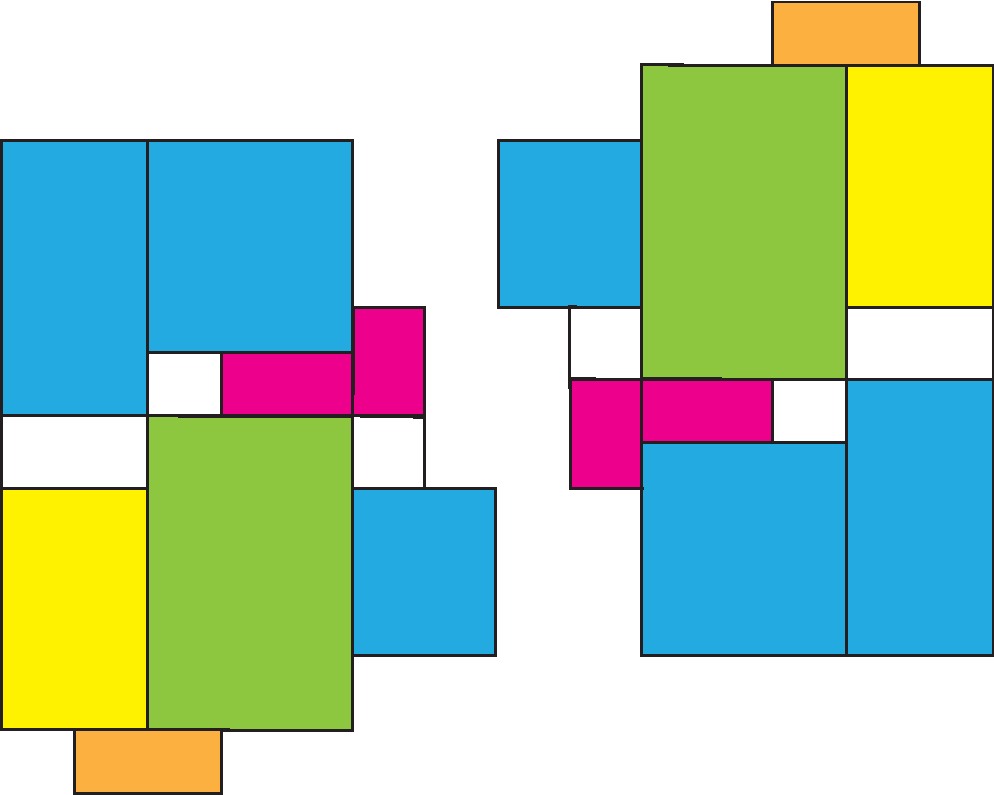
\includegraphics[width=0.37\linewidth]{images/concept2} \hfill
   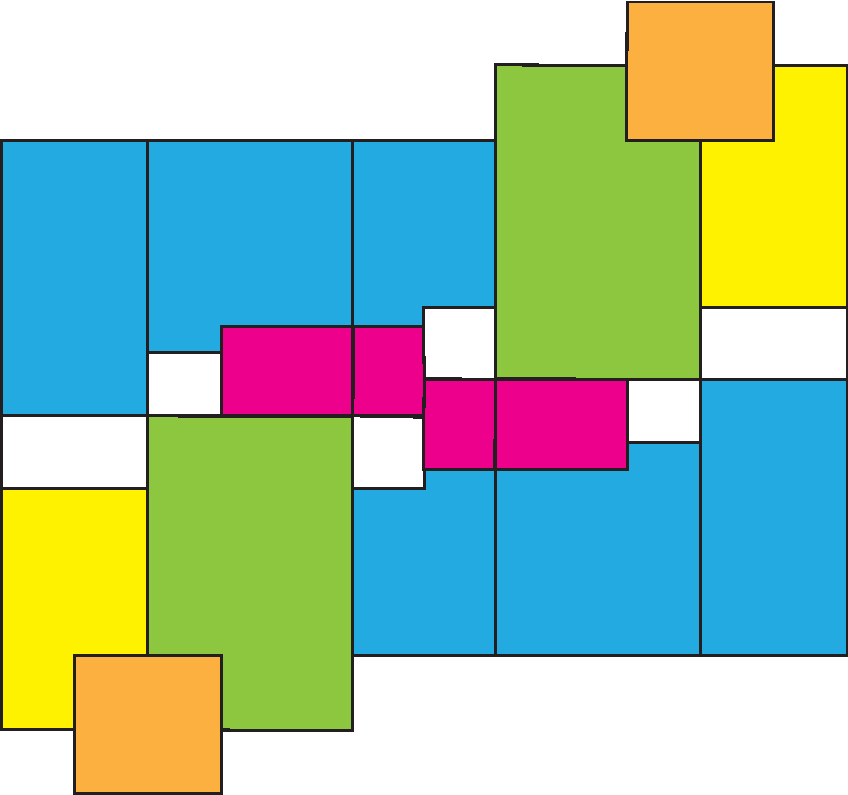
\includegraphics[width=0.32\linewidth]{images/concept3} \hfill
   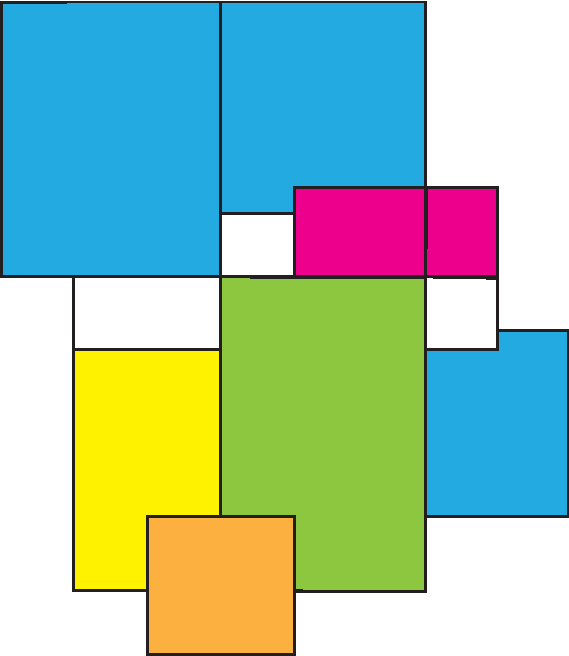
\includegraphics[width=0.215\linewidth]{images/concept0} 
   
   \caption{Concept design. living/eating area (green/yellow); bedrooms (cyan), lavatories (magenta); entrance (white).}
   \label{fig:concept}
\end{figure}

\subsection{LAR model input}


\paragraph{Input of the dwelling concept}
The vertices list \texttt{V} contains pairs of coordinates within a local reference frame. The 2-cell list \texttt{FV}  of references to vertices is given counterclockwise, in order to automatically get a complete LAR representation of topology, i.e.~the pair \texttt{FV, EV} of 2-cells and 1-cells.

%-------------------------------------------------------------------------------
@D Input of LAR architectural plan
@{
V = [[3,-3],
[9,-3],[0,0],[3,0],[9,0],[15,0],
[3,3],[6,3],[9,3],[15,3],[21,3], 
[0,9],[6,9],[15,9],[18,9],[0,13],
[6,13],[9,13],[15,13],[18,10],[21,10], 
[18,13],[6,16],[9,16],[9,17],[15,17],
[18,17],[-3,24],[6,24],[15,24],[-3,13]]
FV = [
[22,23,24,25,29,28], [15,16,22,28,27,30], [18,21,26,25], 
[13,14,19,21,18], [16,17,23,22], [11,12,16,15],
[9,10,20,19,14,13], [2,3,6,7,12,11], [0,1,4,8,7,6,3],
[4,5,9,13,18,17,16,12,7,8],[17,18,25,24,23]]
dwelling = [V,FV]
@}
%-------------------------------------------------------------------------------


\subsection{Partitioning the 1-cells}

The subdivision of 1-cells of the complex between boundary cells and interior cells is executed by computing the boundary operator $\partial_2$, and multiplying it by the coordinate representation $\mathbf{1}$ of the 2D basis of cells. 


\begin{figure}[htbp] %  figure placement: here, top, bottom, or page
   \centering
   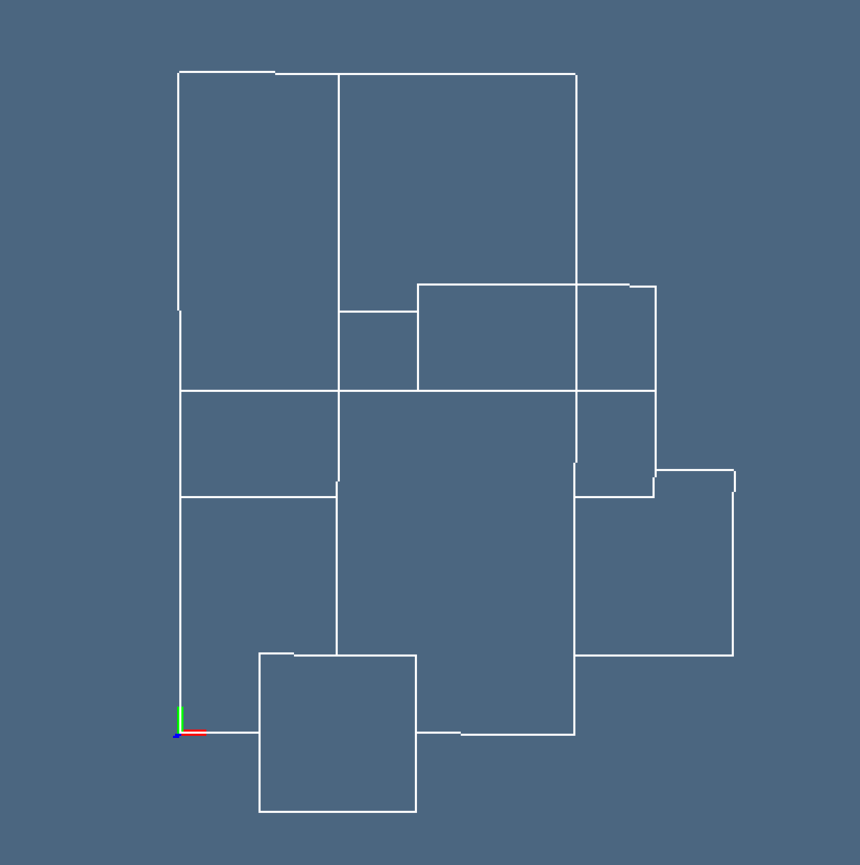
\includegraphics[height=0.243\linewidth,width=0.243\linewidth]{images/plan0} 
   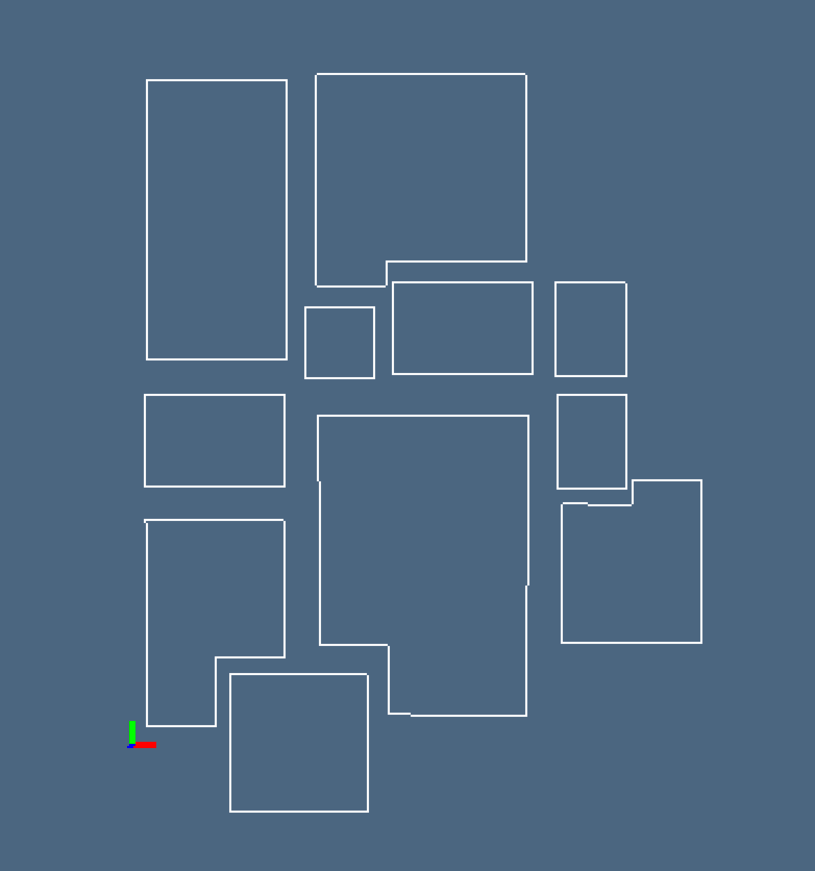
\includegraphics[height=0.243\linewidth,width=0.243\linewidth]{images/plan1} 
   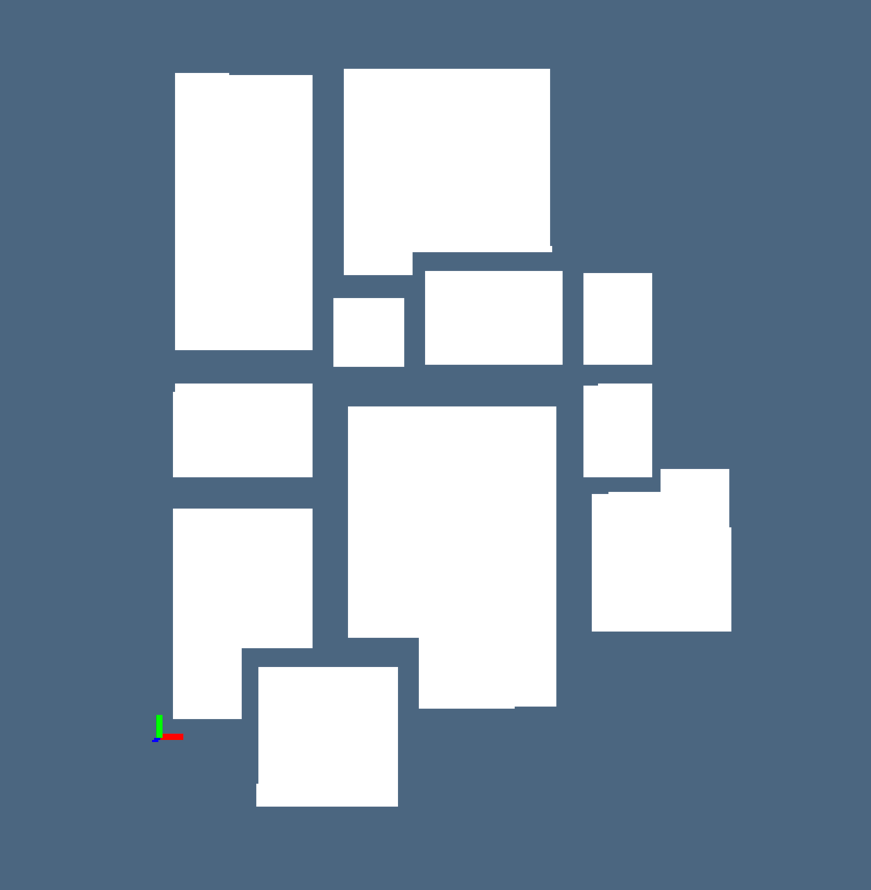
\includegraphics[height=0.243\linewidth,width=0.243\linewidth]{images/plan2} 
   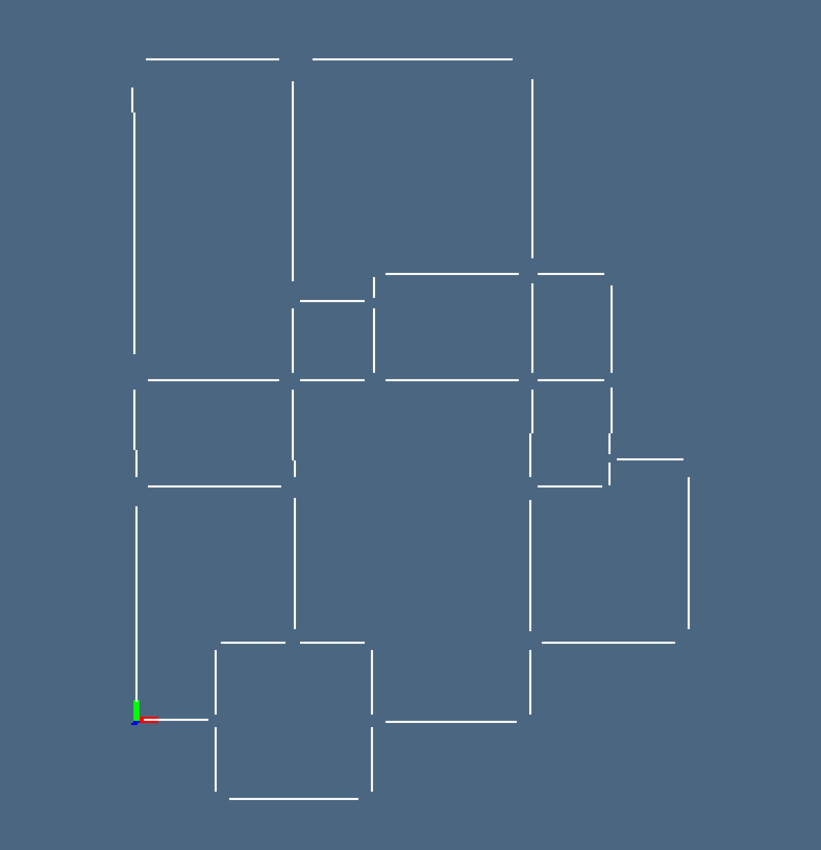
\includegraphics[height=0.243\linewidth,width=0.243\linewidth]{images/plan3} 
   \caption{(a) LAR drawing as close polylines: (b) exploded polylines: (c) exploded 2-cells: (d) exploded 1-cells.}
   \label{fig:plan2D}
\end{figure}

\paragraph{Subdivide the 1-cells of the concept plan}
The input to \texttt{bUnit\_to\_eEiP}, to compute the 1D external envelope and interior partitions starting from 2D from building units, is given below.

%-------------------------------------------------------------------------------
@D Subdivide the 1-cells
@{def bUnit_to_eEiP(FV,EV):
    """ Subdivide the 1-cells. 
    Return external envelope and interior partitions """
    eE = lar2boundaryEdges(FV,EV)
    iP = lar2InteriorEdges(FV,EV)
    return eE,iP
@}
%-------------------------------------------------------------------------------


\begin{figure}[htbp] %  figure placement: here, top, bottom, or page
   \centering
   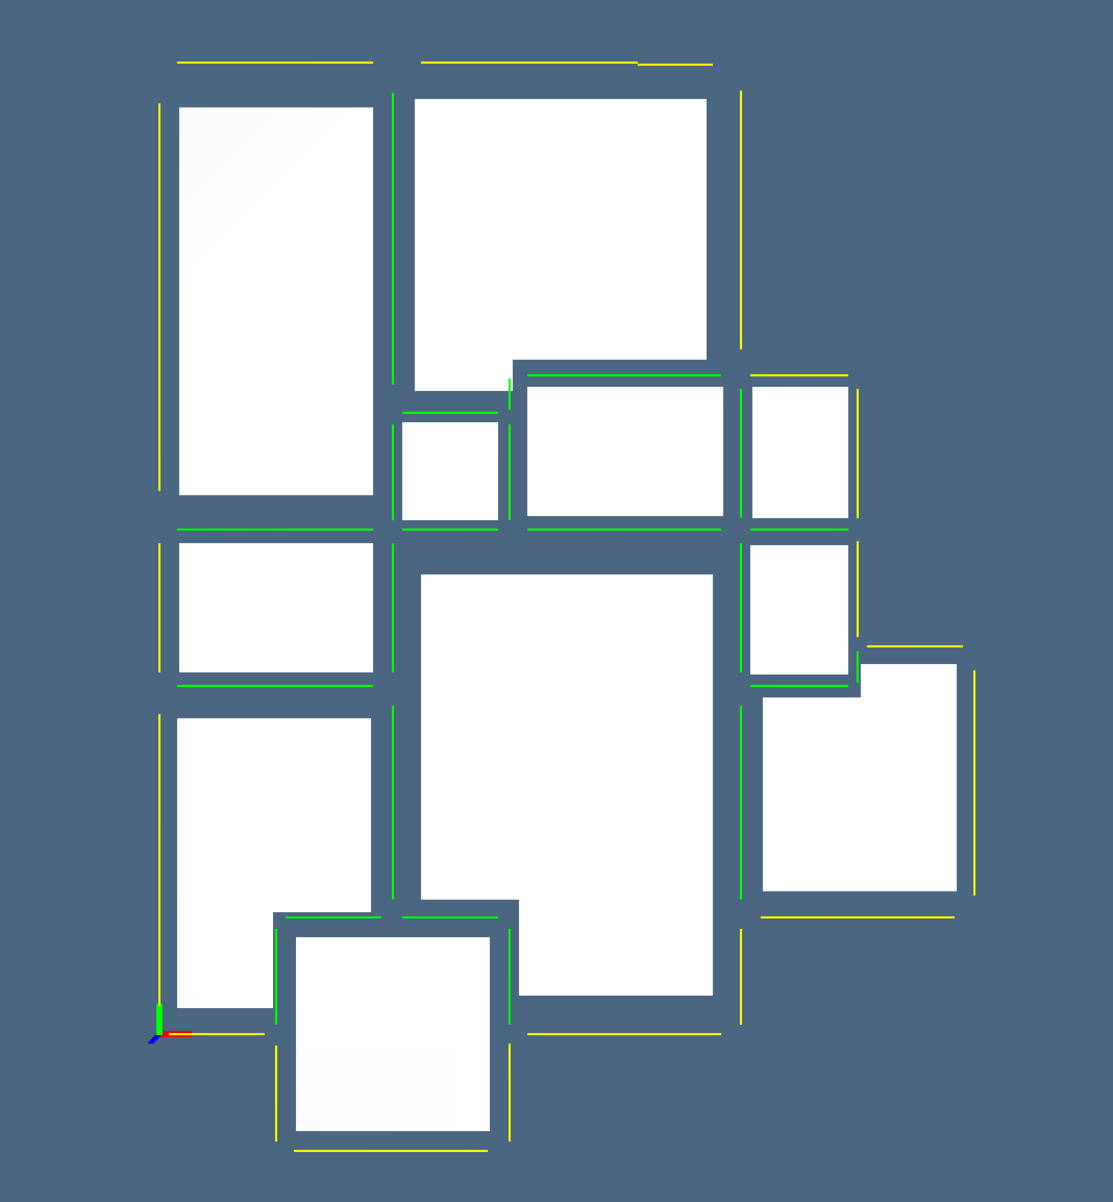
\includegraphics[height=0.325\linewidth,width=0.325\linewidth]{images/plan4} 
   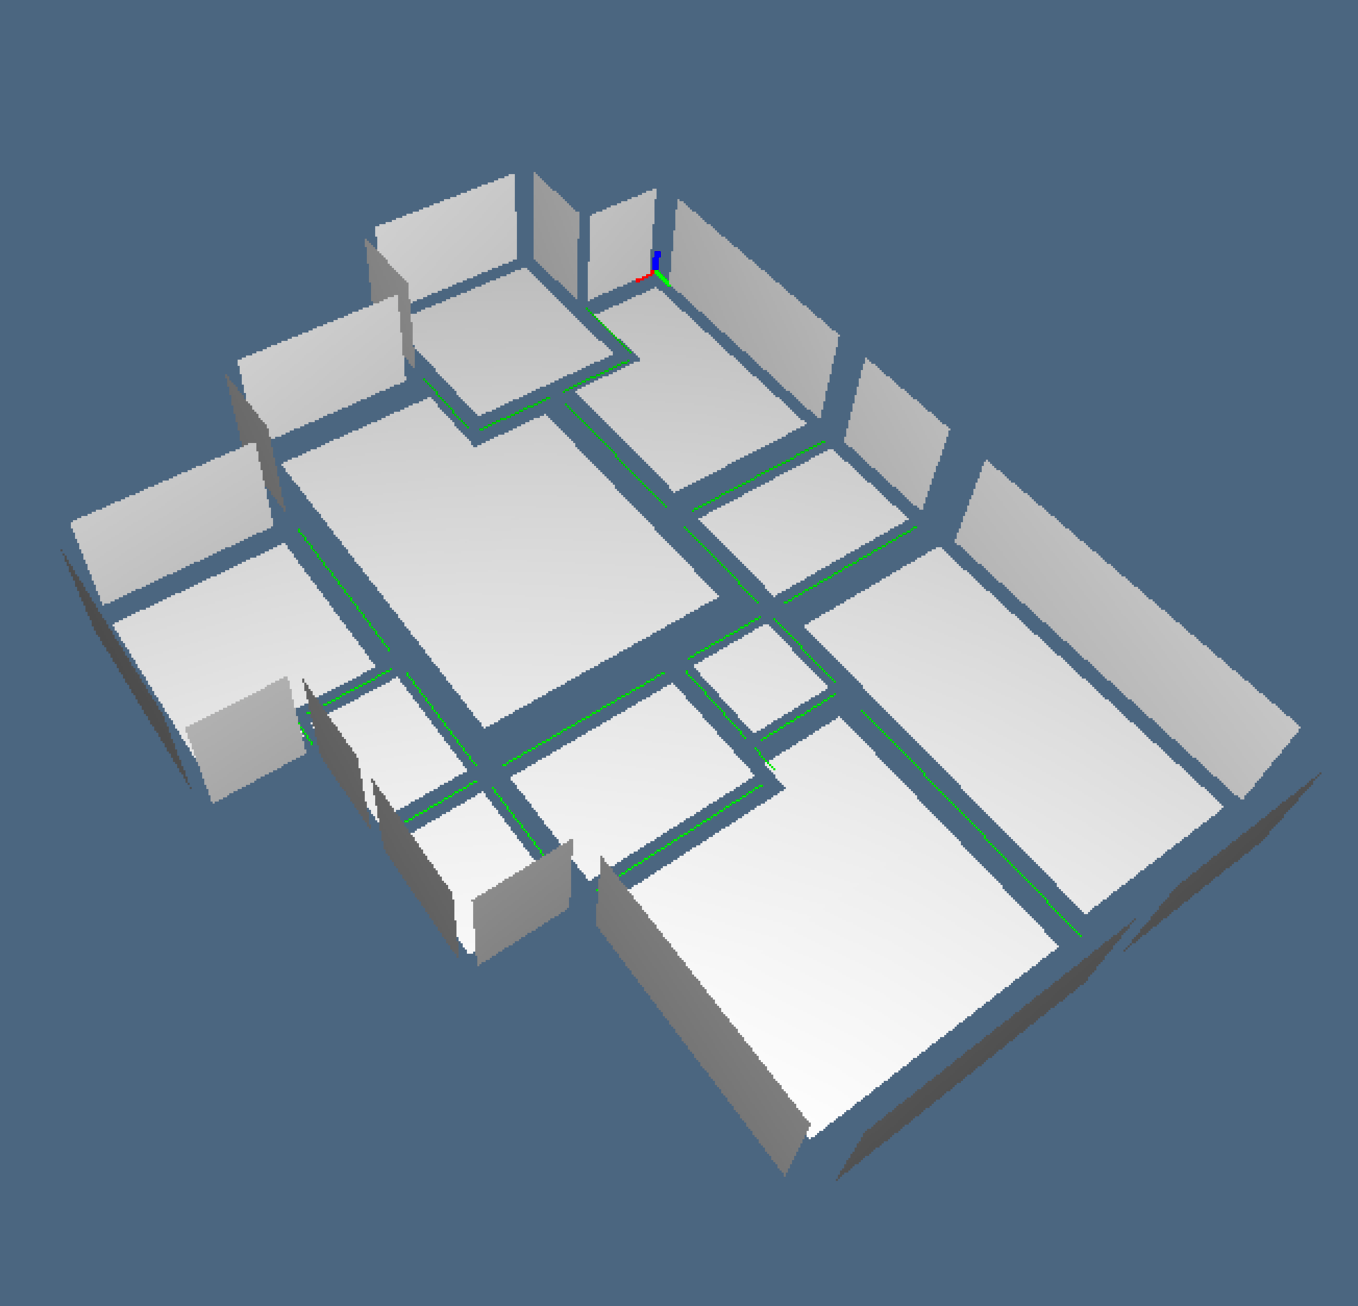
\includegraphics[height=0.325\linewidth,width=0.325\linewidth]{images/plan5} 
   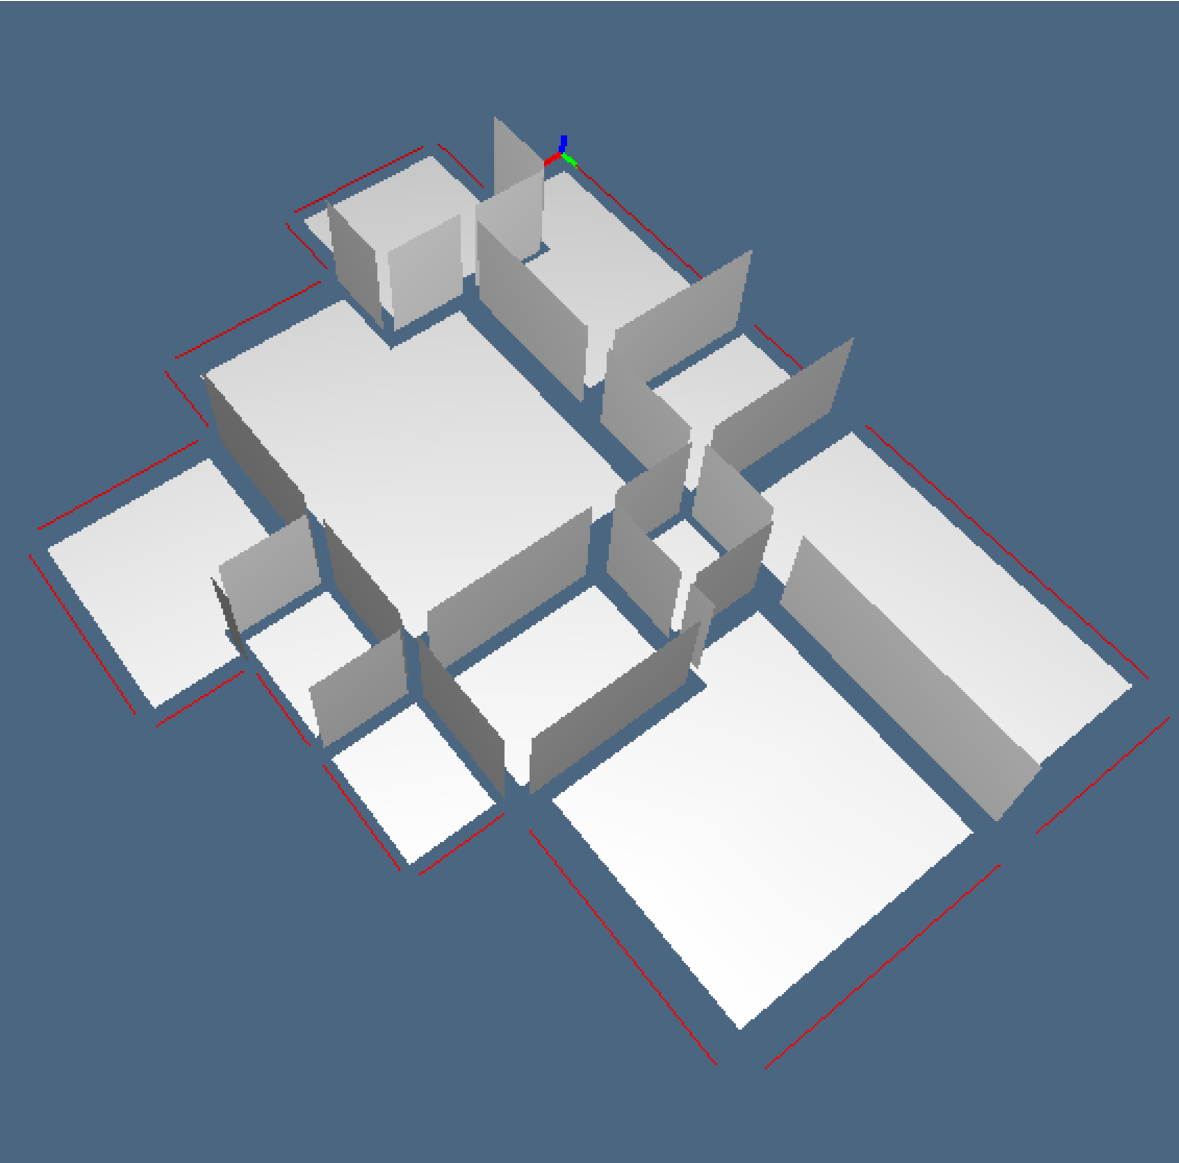
\includegraphics[height=0.325\linewidth,width=0.325\linewidth]{images/plan6} 
   \caption{(a) 2-cells, interior 1-chain (green), boundary 1-chain (red): (b) boundary 2-chain: (c) interior 2-chain.}
   \label{fig:plan2.5D}
\end{figure}


\begin{figure}[htbp] %  figure placement: here, top, bottom, or page
   \centering
   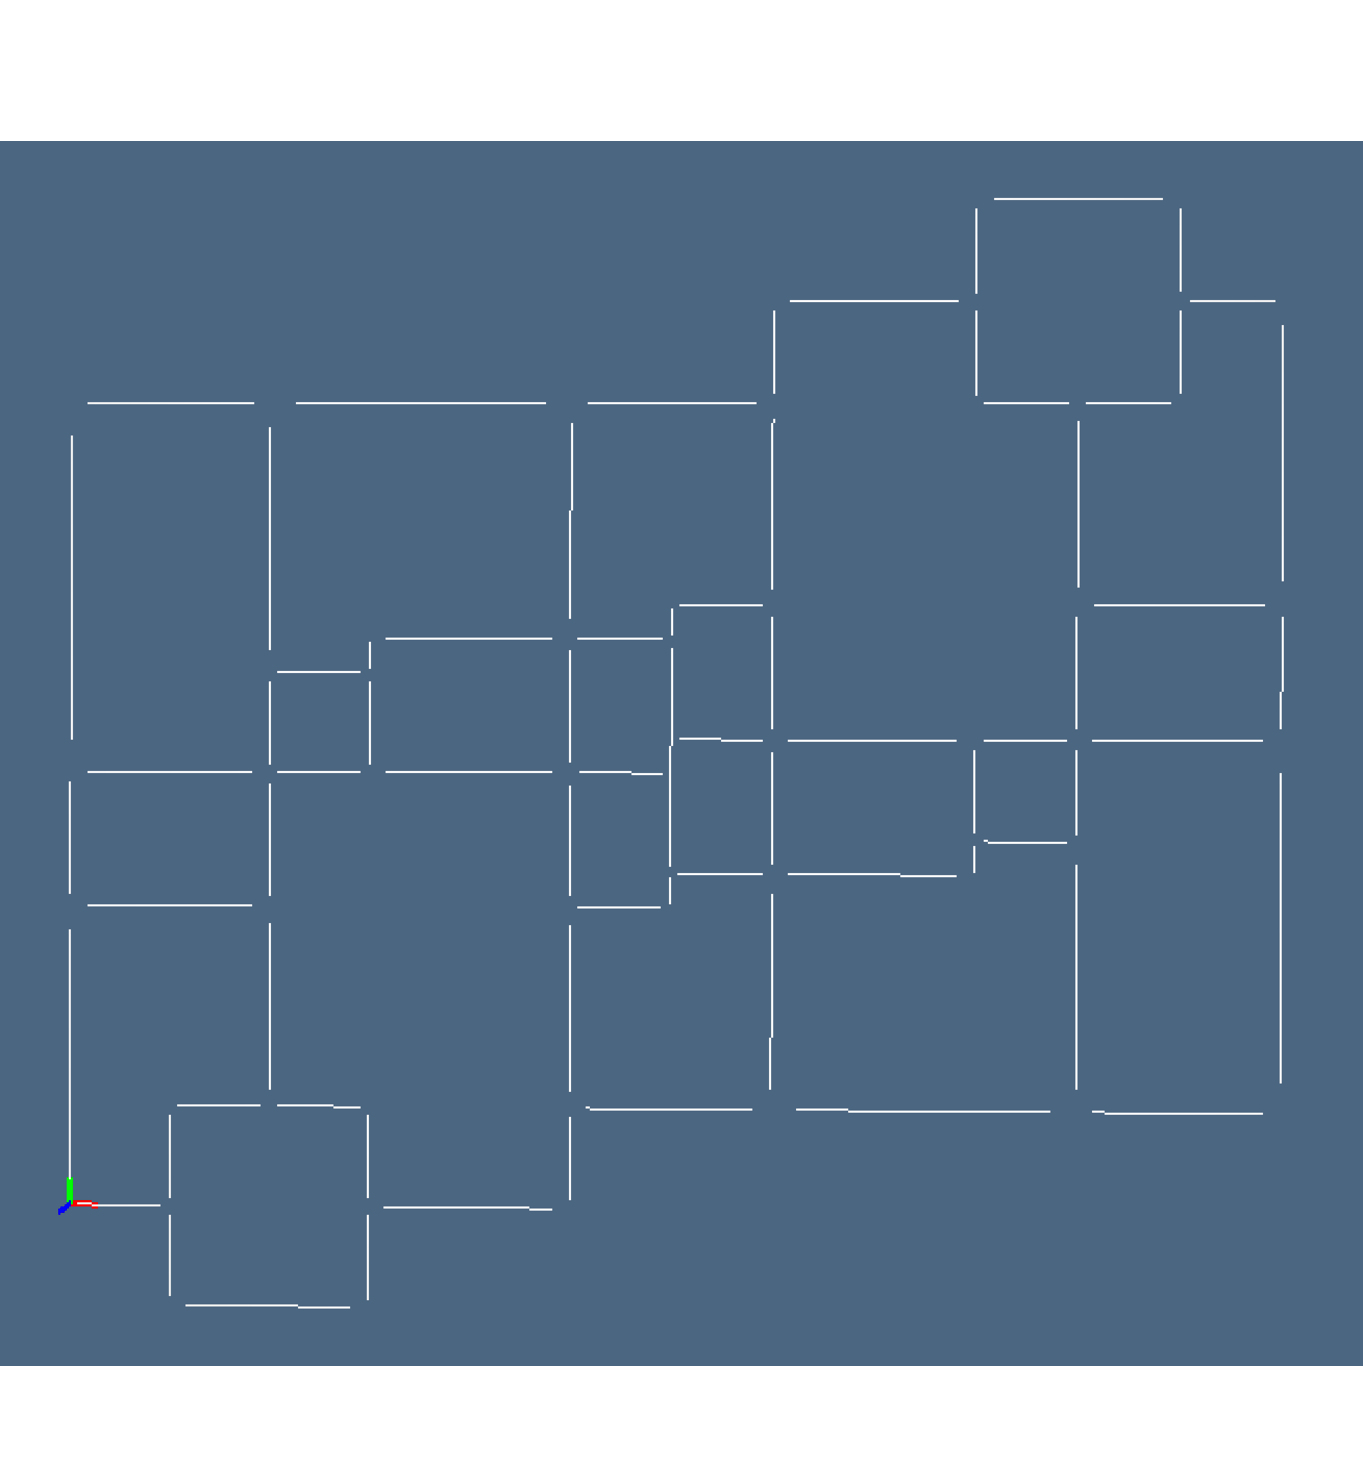
\includegraphics[width=0.33\linewidth]{images/planpair} 
   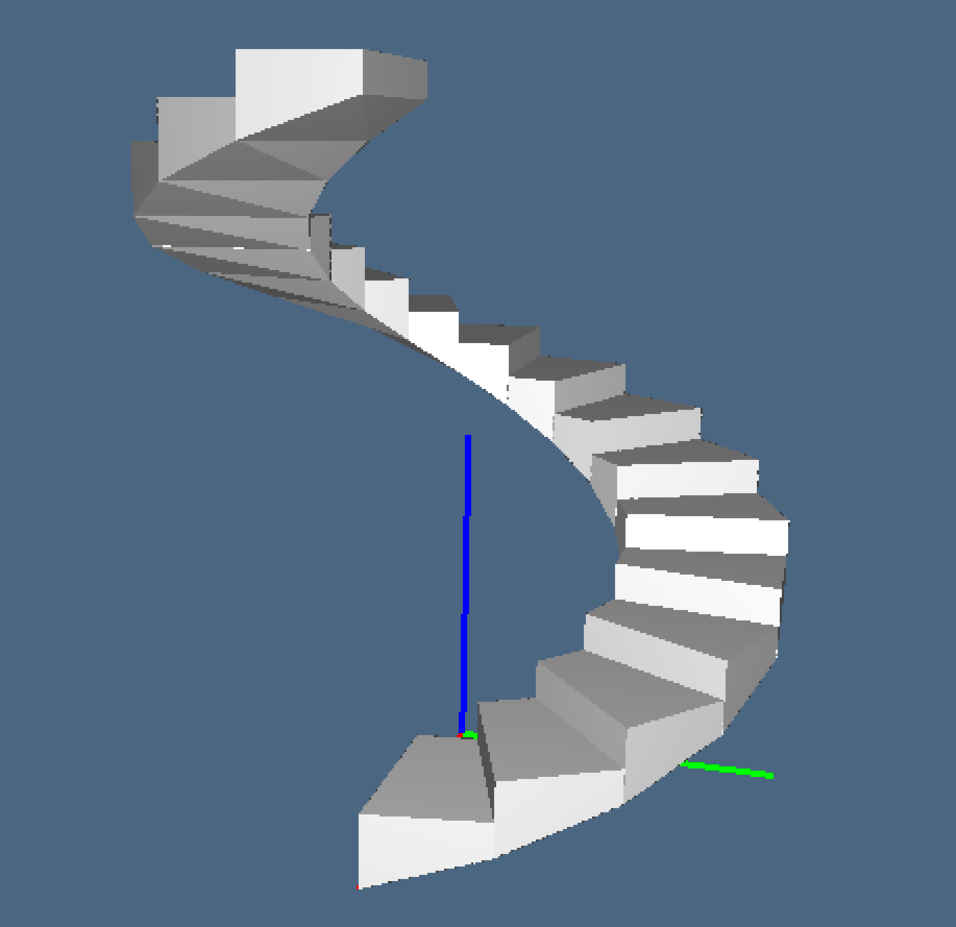
\includegraphics[width=0.3\linewidth]{images/spiralstair} 
   \caption{Concept design: (a) aggregation of two building units; (b) fully parametric spiral stair.}
   \label{fig:concept1}
\end{figure}

\subsection{Floor assembly of apartment building}

\begin{figure}[htbp] %  figure placement: here, top, bottom, or page
   \centering
   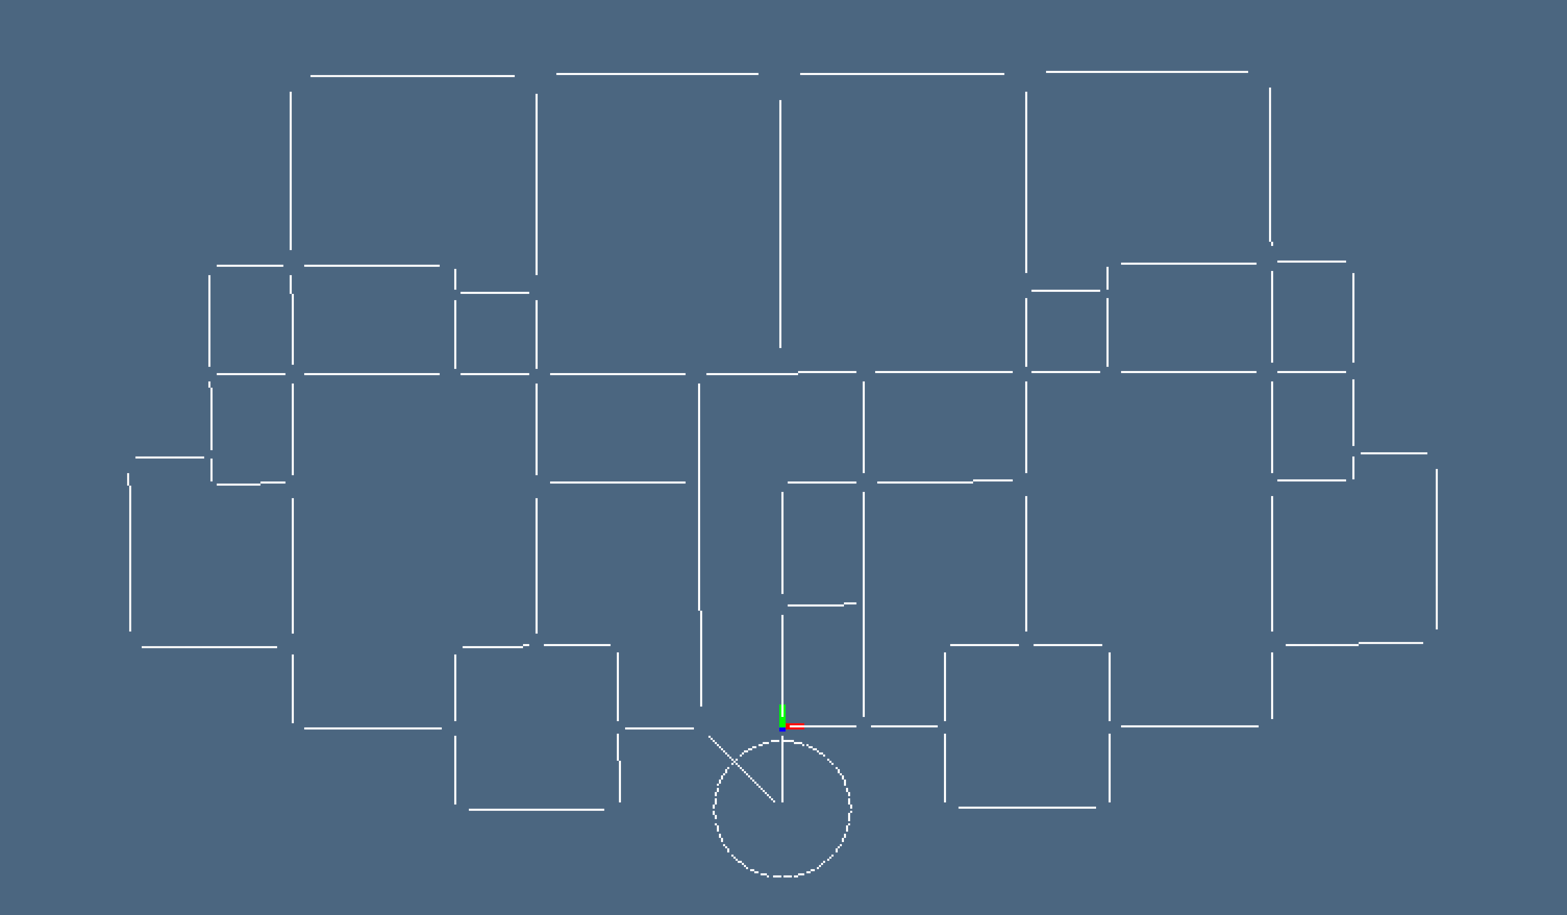
\includegraphics[width=0.6\linewidth]{images/plan2d} 
   \caption{Concept design: (a) aggregation of two building units; (b) fully parametric spiral stair.}
   \label{fig:concept1}
\end{figure}

\paragraph{Typical floor assembly of apartment block}

%-------------------------------------------------------------------------------
@O test/py/architectural/test04.py
@{""" D LAR model input and handling """
@< Initial import of modules @>
@< Input of LAR architectural plan @>
@< Generation of the typical flat of apartment block @>
@}
%-------------------------------------------------------------------------------

%-------------------------------------------------------------------------------
@D Generation of the typical flat of apartment block
@{V,FV = larApply(t(3,0))(dwelling)
print "\n V,FV =",V,FV
VIEW(EXPLODE(1.2,1.2,1)(MKPOLS(dwelling)))
dwelling = Struct([ t(3,0), dwelling ])
V1 = [[0,0],[3,0],[3,4.5],[0,4.5],[3,9],[0,9],[3,13],[-3,13],[-3,0],[0,-3]]
FV1 = [[0,1,2,3],[3,2,4,5],[0,3,5,4,6,7,8,9]]
landing = V1,FV1
plan = Struct([landing,dwelling,s(-1,1),dwelling])
assembly2D = evalStruct(plan)
assembly1D = larCells(face2edge)(assembly2D)
VIEW(EXPLODE(1.2,1.2,1)(CAT(AA(MKPOLS)(assembly1D))))
@}
%-------------------------------------------------------------------------------




\paragraph{Initial 3D assembly of apartment block}

%-------------------------------------------------------------------------------
@O test/py/architectural/test05.py
@{""" 3D mock-up of apartment block """
@< Initial import of modules @>
@< Input of LAR architectural plan @>
@< Generation of the typical flat of apartment block @>
stair = spiralStair(width=0.2,R=3,r=0.25,riser=0.1,pitch=4.4,nturns=1.75,steps=36)
stair = larApply(r(0,0,3*PI/4))(stair)
stair = larApply(t(0,-3,0))(stair)
stairColumn = larApply(t(0,-3,0))(larRod(0.25,4.2)())
mod_1 = larQuote1D( 6*[0.2,-3.8] )
assembly3D = larBinOps(larModelProduct)(assembly2D)(mod_1)
VIEW(EXPLODE(1.2,1.2,1)(CAT(AA(MKPOLS)(assembly3D))))

horClosures = horizontalClosures([0.2,-3.8]*12 +[0.2])(assembly2D)
VIEW(STRUCT(horClosures))

wire = SKEL_1(INSR(PROD)(AA(QUOTE)([[6,9,9,9,9,6],[-3,10,11],[4]*12])))
VIEW(wire)
frame3D = T(1)(-24)(OFFSET([.2,.6,.2])(wire))
VIEW(frame3D)

assembly3D = evalStruct(Struct([stairColumn,stair,t(0,0,4)]*12))
VIEW(STRUCT(CAT(AA(MKPOLS)(assembly3D)) + horClosures + [frame3D]))
@}
%-------------------------------------------------------------------------------


%-------------------------------------------------------------------------------
@O test/py/architectural/test01.py
@{""" test file """
@< Initial import of modules @>
@< Input of LAR architectural plan @>
bU = AA(SOLIDIFY)(AA(POLYLINE)(lar2polylines (dwelling)))
EV = face2edge(FV)
VIEW(EXPLODE(1.2,1.2,1)(MKPOLS((V,EV))))

eE,iP = bUnit_to_eEiP(FV,EV)
modEe1D = V, [EV[e] for e in eE]
modIp1D = V, [EV[e] for e in iP]
eE1D = AA(COLOR(RED))(MKPOLS(modEe1D))
iP1D = AA(COLOR(GREEN))(MKPOLS(modIp1D))

VIEW(EXPLODE(1.2,1.2,1)(eE1D))
VIEW(EXPLODE(1.2,1.2,1)(iP1D))
VIEW(STRUCT(bU + iP1D + eE1D))
VIEW(EXPLODE(1.2,1.2,1)(bU + iP1D + eE1D))

floorHeight = larIntervals([1])([4])
modIp2D = larModelProduct([ modIp1D, floorHeight ])
modEe2D = larModelProduct([ modEe1D, floorHeight ])

VIEW(EXPLODE(1.2,1.2,1)(bU + MKPOLS(modIp2D) + eE1D))
VIEW(EXPLODE(1.2,1.2,1)(bU + iP1D + MKPOLS(modEe2D)))
VIEW(EXPLODE(1.2,1.2,1)(bU + MKPOLS(modIp2D) + MKPOLS(modEe2D)))
@}
%-------------------------------------------------------------------------------


\paragraph{Horizontal closures generator}
The function \texttt{horizontalClosures} is applied to a 2D assembly and to a 1D pattern of positive (full) or negative (empty) measures, in order to generate a 3D model of vertical closures of a building block.

%-------------------------------------------------------------------------------
@D Horizontal closures generator
@{def horizontalClosures(pattern):
    vertical1D = larQuote1D(pattern)
    vertical0D = larQuote0D(pattern)
    def horizontalClosures0(assembly2D):
        out = []
        for flat2D in assembly2D:
            V,FV = flat2D
            EV = face2edge(FV)
            dwellH3D = larModelProduct([flat2D,vertical0D])
            dwellV3D = larModelProduct([(V,EV),vertical1D])
            poly3D = AA(POLYLINE)(lar2polylines(dwellH3D))
            floors3D = AA(solidify)(poly3D)
            out += floors3D+MKPOLS(dwellV3D)
        return out
    return horizontalClosures0
@}
%-------------------------------------------------------------------------------



\paragraph{Spatial beams and frames}
%-------------------------------------------------------------------------------
@D Spatial beams and frames
@{""" Spatial beams and frames """
columns0D = V,[[k] for k in range(len(V))]
columns = larModelProduct([columns0D,larQuote1D([4])])
indices = [T([1,2])(v)(S([1,2])([.1,.1])(TEXT(str(k)))) for k,v in enumerate(V)]
VIEW(STRUCT(MKPOLS(columns)+indices))

wire = SKEL_1(INSR(PROD)(AA(QUOTE)([[6,9,9,9,9,6],[-3,10,11],[4.2]*5])))
VIEW(wire)
frame3D = T(1)(-24)(OFFSET([.2,.4,.4])(wire))
VIEW(frame3D)
@}
%-------------------------------------------------------------------------------

%===============================================================================
\section{Test case: generation of 3D model of tower building}\label{sec:library}
%===============================================================================

The generation (and visualization) of a business tower building is produced in this section, starting from a wire-frame vector drawings of typical floorplan. A movie file of the whole generation is given in \href{http://paoluzzi.dia.uniroma3.it/web/filmato.mov}{http://paoluzzi.dia.uniroma3.it/web/filmato.mov}.

The movie begins from a graphical editor (in this case Adobe Illustrator) showing the content of a  raster file  within the session canvas, with a PNG image of a typical floor plan of the tower building. Then a second layer is shown, superimposing a vector drawing traced with red gross lines, and without precision at the crossings of lines. This fact is made evident by some zoom-ins. 

Then the movie presents the only layer showing the vector drawing obtained as simplified "wire-frame"  tracing of the original raster image. This drawing is saved as SVG file, the W3C format for vector graphics on the web.

The crossing points of lines will be precisely computed by the server application, discussed in the following sections, that is written in python using \href{https://github.com/plasm-language/pyplasm}{pyplasm} and \href{https://github.com/cvdlab/lar-cc}{larlib}.


Adobe Illustrator is then left, and the movie shows the command-line terminal and the Python sources of the application within a text editor. The code is written in a very general form, but with some \emph{ad-hoc} customizations intended only for this test-case. These will be substituted by interactive operations on the graphical UI, when developed. Such customizations are used here to identify the 2-cells to consider "empty space" (i.e.~stairs and elevators). In the following we discuss the application code.

%-------------------------------------------------------------------------------
\subsection{Input of floorplan wire-frame}
%-------------------------------------------------------------------------------

First the \texttt{larlib} modules are imported, and the \texttt{plan.svg} file is read from the \texttt{test/inters} subdirectory.
Then the parsed contents are handled by the \texttt{svg2lar} function, producing a first \texttt{larModel}.

\paragraph{Input of floorplan wire-frame}
%-------------------------------------------------------------------------------
@D Input of floorplan wire-frame
@{""" import modules from larlib """
from larlib import *

""" Input of floorplan wire-frame """
filename = "test/svg/inters/plan.svg"
larModel = svg2lar(filename)
@}
%-------------------------------------------------------------------------------

%-------------------------------------------------------------------------------
\subsection{Generation of 2-cellular complexes}
%-------------------------------------------------------------------------------

Here we produce the first visualization of the test-case application, showing a well-formed cellular  2-complex, i.e.~a planar embedding of a graph. \texttt{V,FV,EV} are the components of a standard LAR format, after that the biconnected components of the plan graph have beeen computed, and the ``dangling'' edges and trees have been removed.
The 0-cells (vertices), 1-cells (edges) and 2-cells (faces) are numbered according to position in their arrays (see Figure~\ref{fig:towerplan1}).
From now on LAR provides a complete support and control of layout topology.

\begin{figure}[htbp] %  figure placement: here, top, bottom, or page
   \centering
   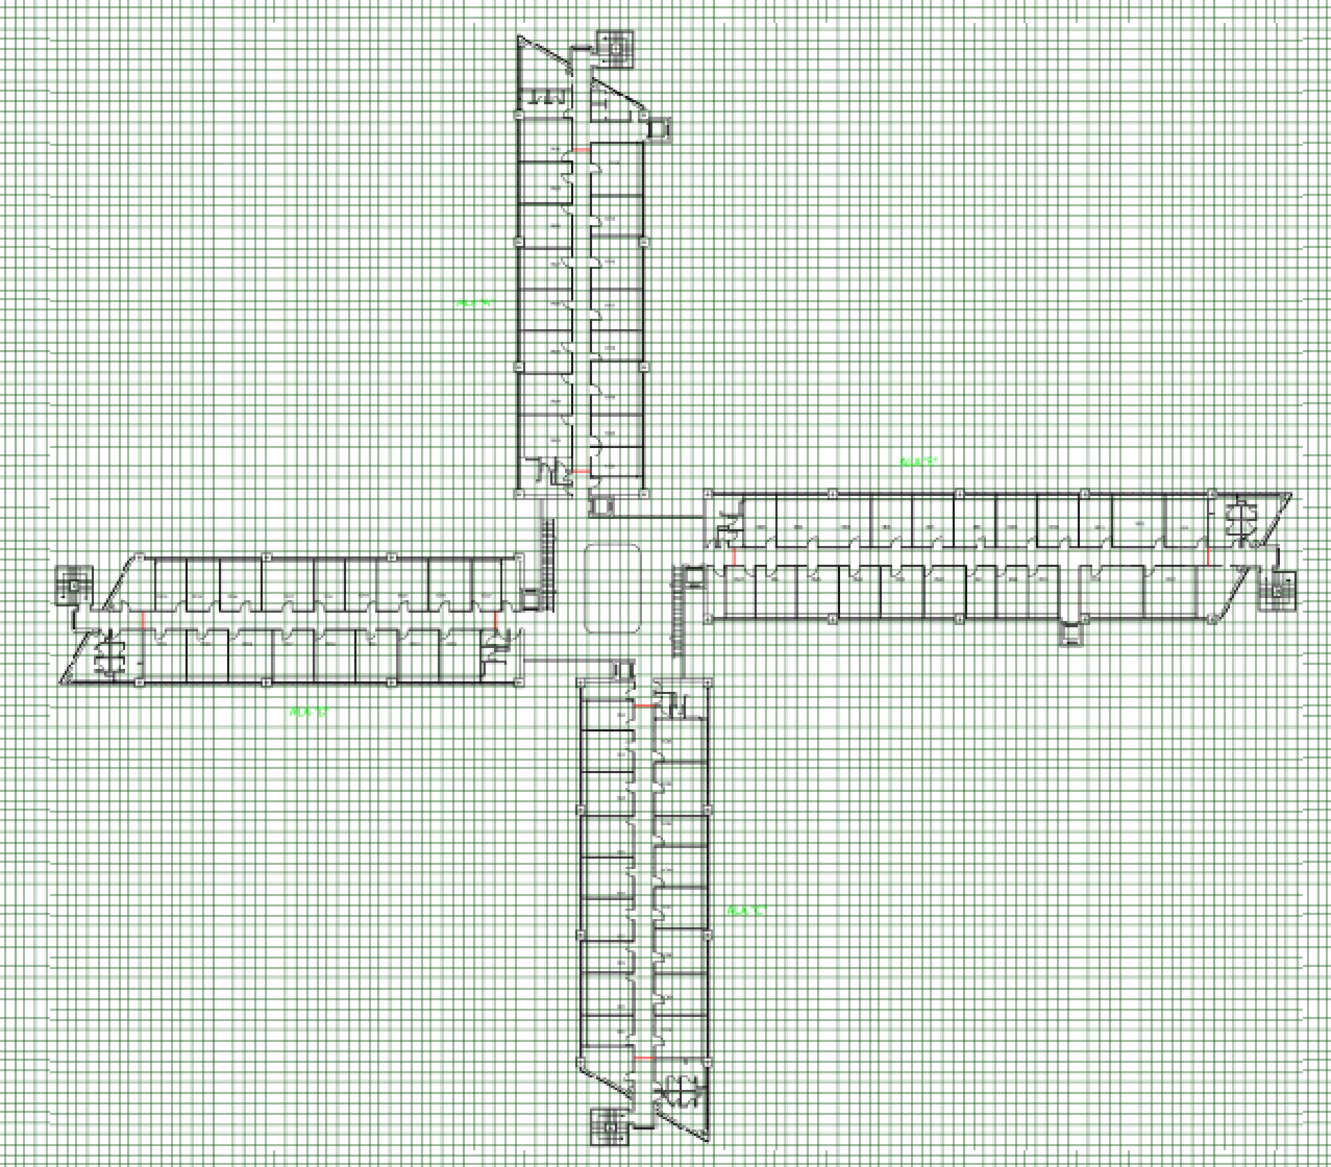
\includegraphics[width=0.325\linewidth]{images/towerplan0} 
   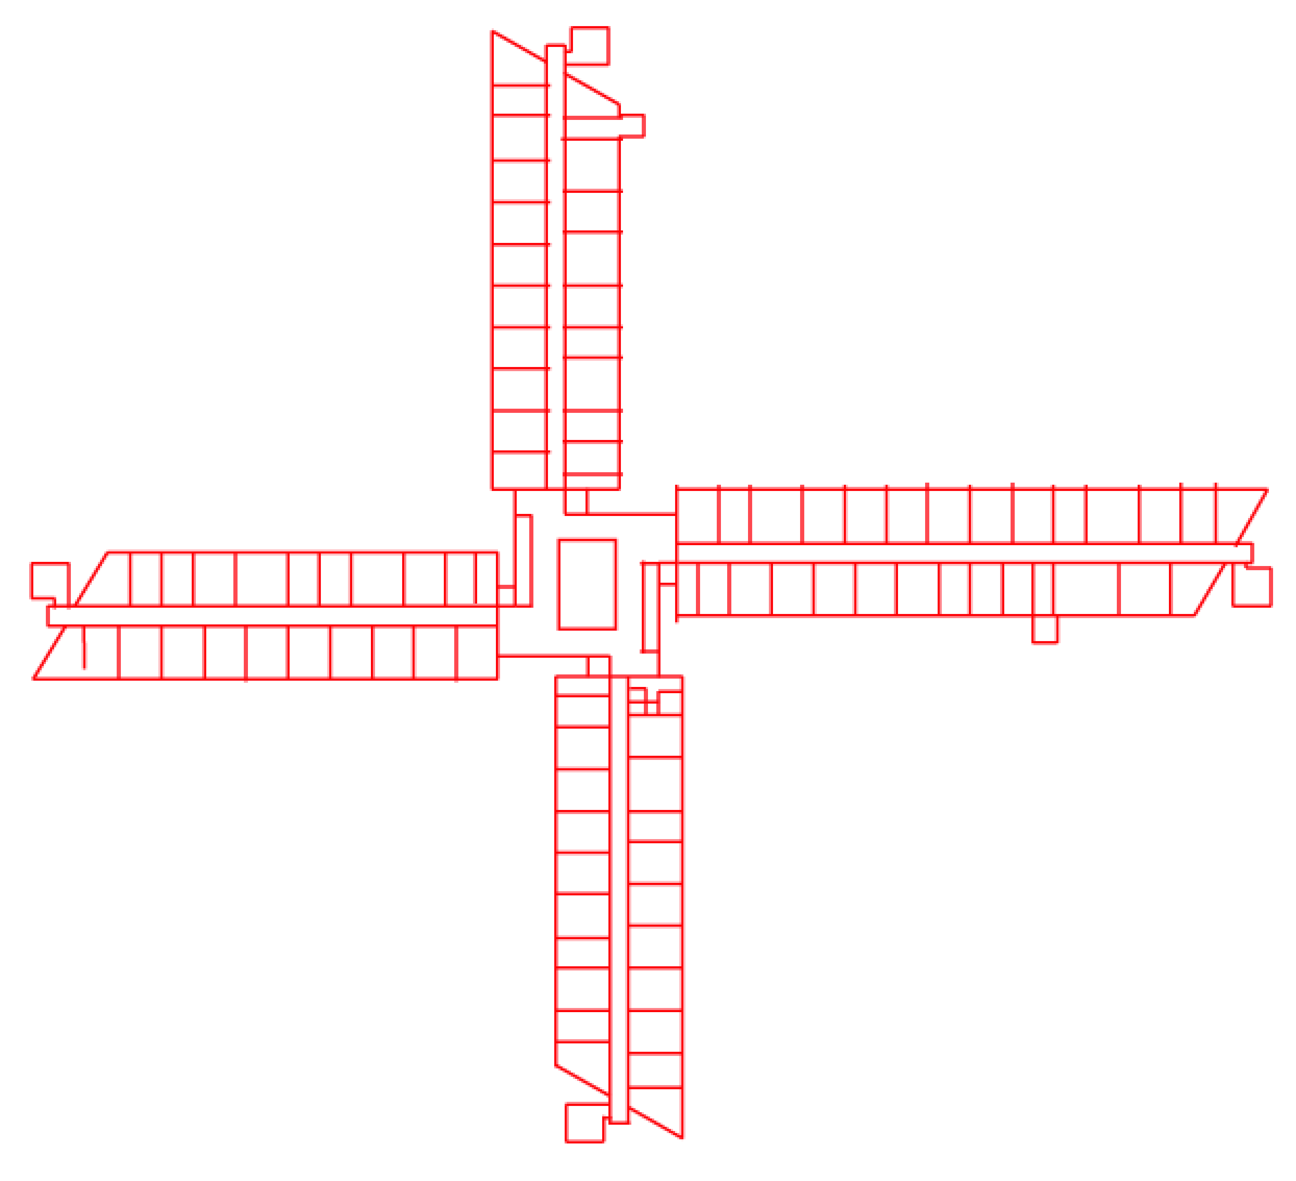
\includegraphics[width=0.325\linewidth]{images/towerplan2} 
   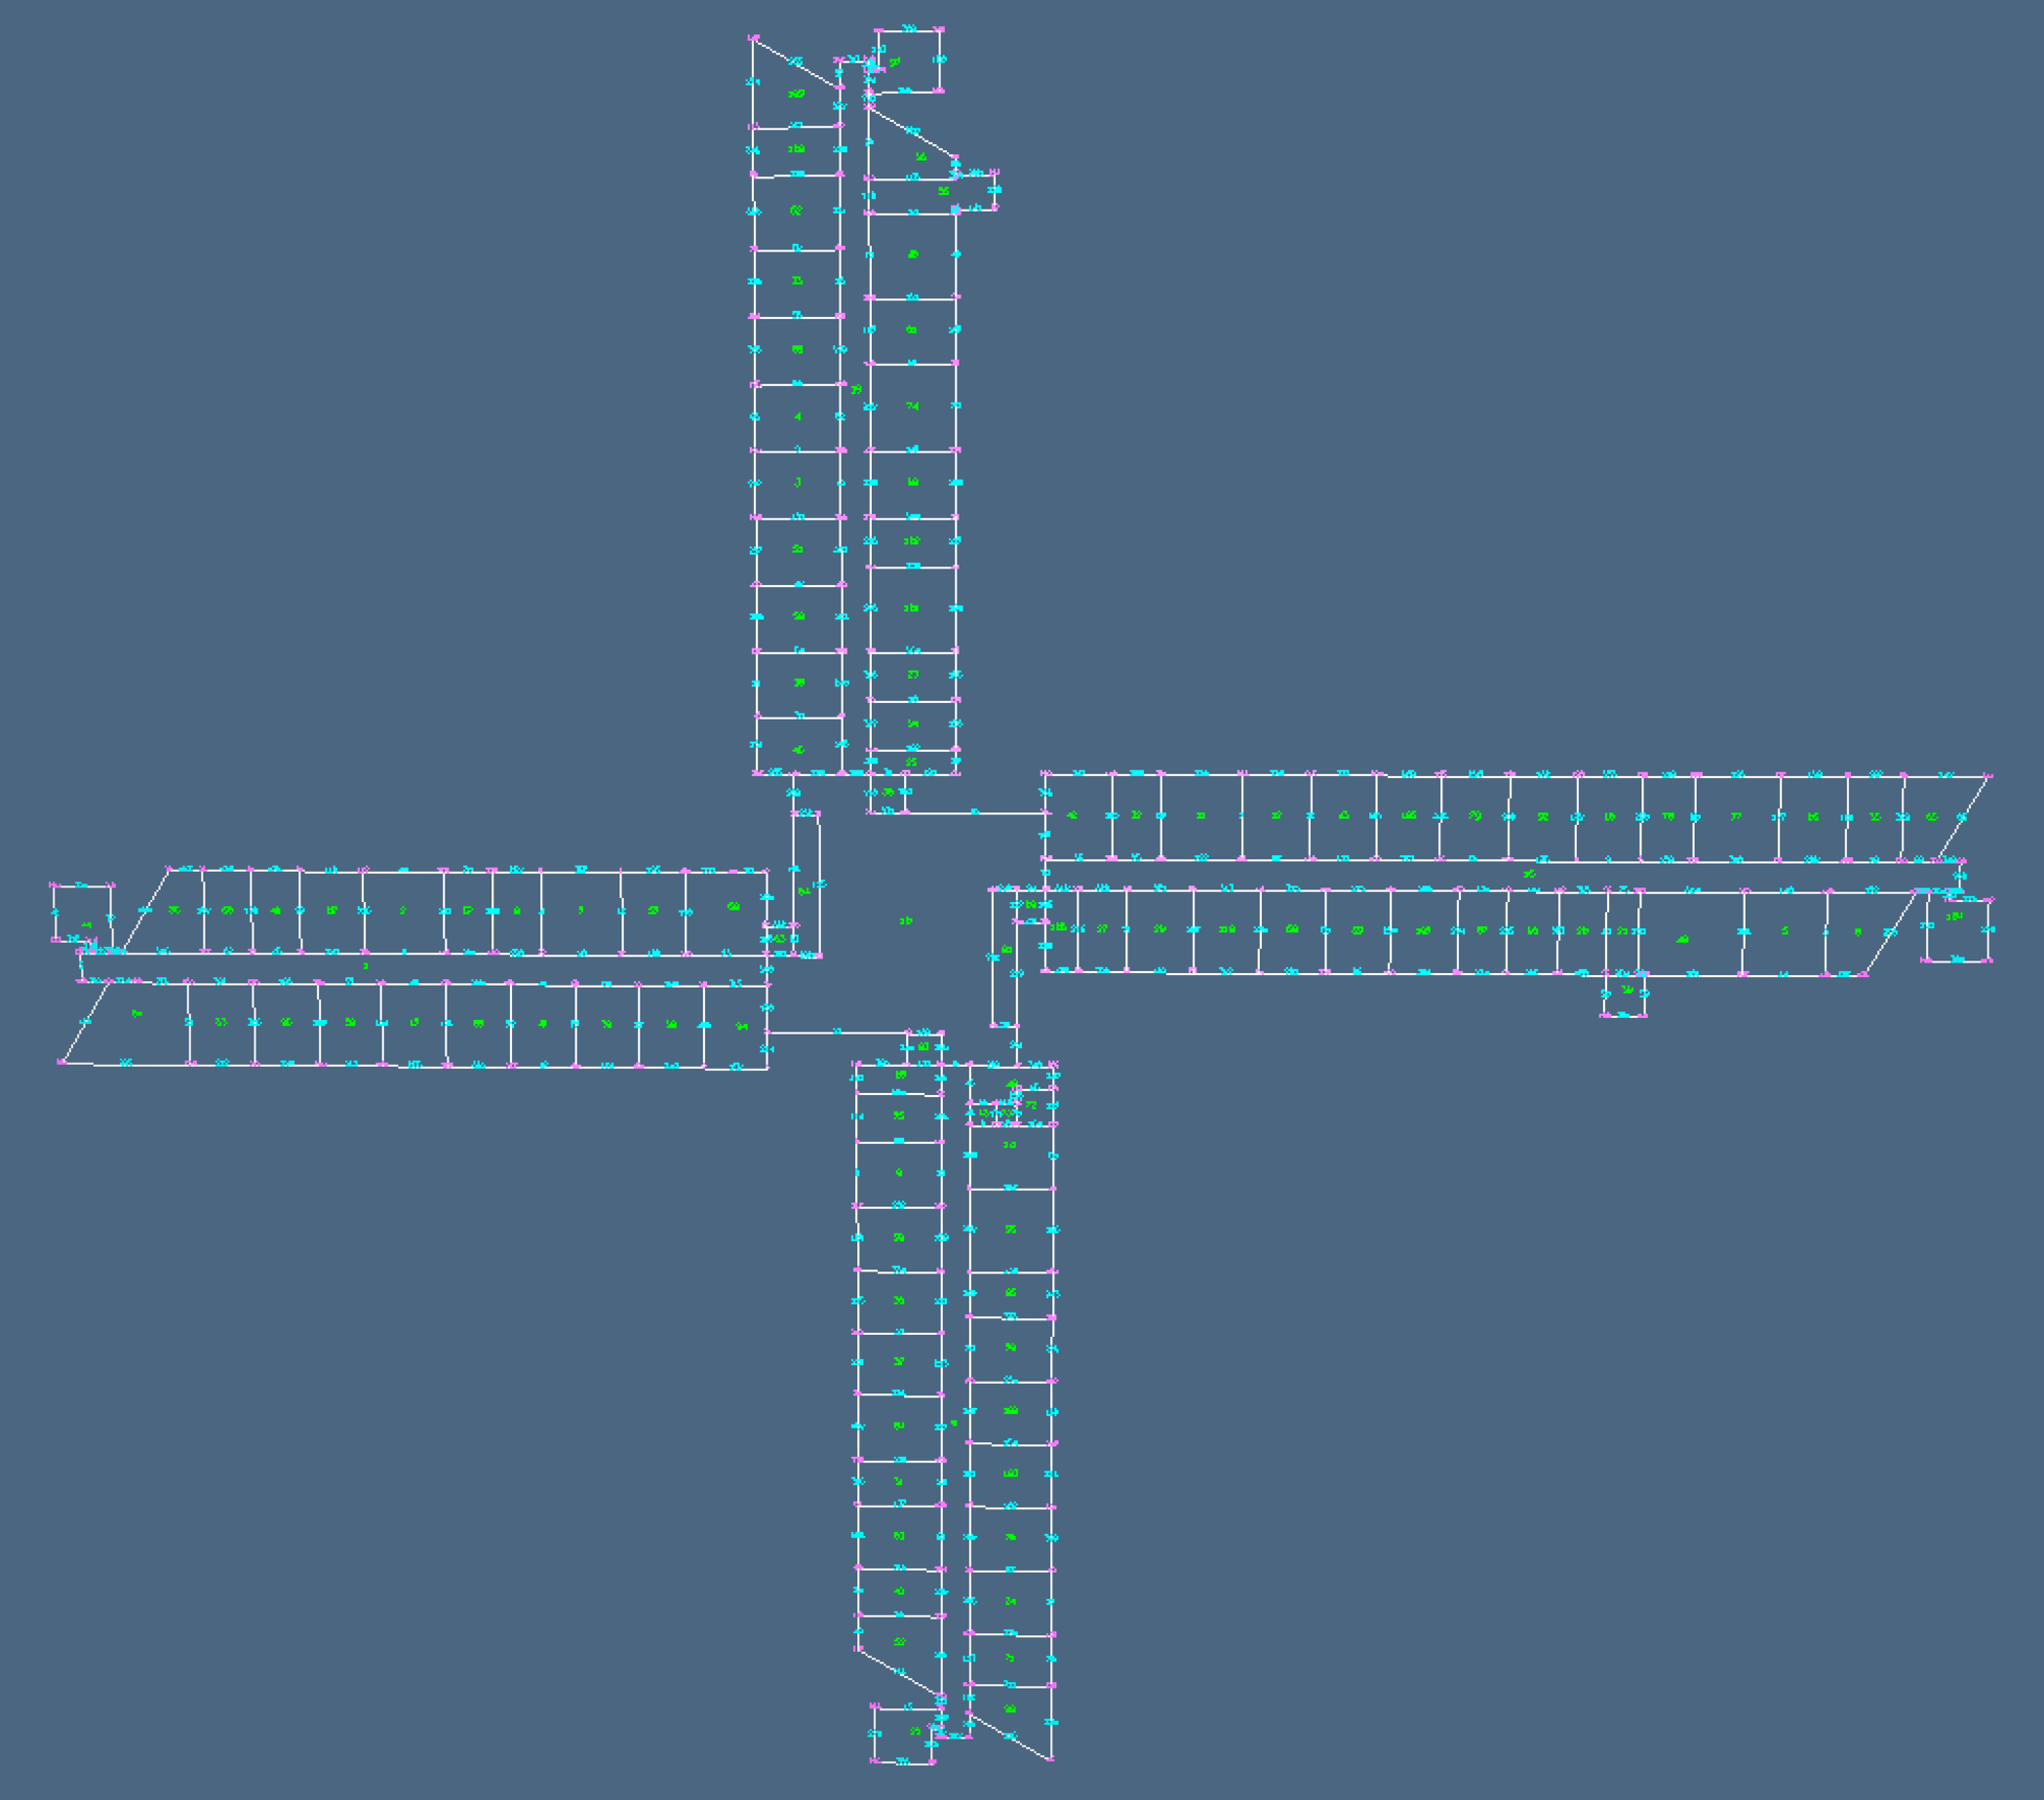
\includegraphics[width=0.325\linewidth]{images/towerplan1} 
   \caption{(a) The input raster floorplan; (b) the vector ``wire-frame'' drawing; (c) the computed cellular 2-complex.}
   \label{fig:towerplan1}
\end{figure}

\paragraph{Generation of 2-cellular complexes}
The value of \texttt{scaleFactor} was precomputed to transform the model to unit sizes.
%-------------------------------------------------------------------------------
@D Generation of 2-cellular complexes
@{""" Generation of 2-cellular complexes """

""" Floor layout generation as LAR cellular complex """
scaleFactor = 83.333
larModel = larApply(s(scaleFactor,scaleFactor))(larModel)
V,FV,EV = larModel

""" Visualization of cell numbering of floorplan 2-complex """
VV = AA(LIST)(range(len(V)))
submodel = STRUCT(MKPOLS((V,EV)))
VIEW(larModelNumbering(1,1,1)(V,[VV,EV,FV[:-1]],submodel,2.5))
@}
%-------------------------------------------------------------------------------

%-------------------------------------------------------------------------------
\subsection{Selection of specialized 1-chains}
%-------------------------------------------------------------------------------

Three types of 1-chains are computed, corresponding to the subsets of boundary edges, corridor edges but the boundary ones; and  internal edges (but corridor edges). The latter correspond to the building components (blind walls) without openings; the former to the building enclosures, where windows will be automatically open. The corridor edges are used to automatically open the doors.

\paragraph{Selection of specialized 1-chains}
%-------------------------------------------------------------------------------
@D Selection of specialized 1-chains
@{""" Selection of specialized 1-chains """

""" Classification of edges (boundary, interior, passage 1-chains) """
FE = crossRelation(FV,EV)
boundaryEdges = boundaryCells(FV[:-1], EV)
corridorEdges = list(set(CAT([FE[k] for k in [1,16,9,19,10]])).difference(boundaryEdges))
internalEdges = set(range(len(EV))).difference(boundaryEdges+corridorEdges)

boundaryWalls = AA(COLOR(CYAN))(MKPOLS((V,[EV[k] for k in boundaryEdges])))
internalWalls = AA(COLOR(MAGENTA))(MKPOLS((V,[EV[k] for k in internalEdges])))
corridorWalls = AA(COLOR(YELLOW))(MKPOLS((V,[EV[k] for k in corridorEdges])))

""" Visualization of coloured chains """
submodel = STRUCT(boundaryWalls+internalWalls+corridorWalls)
VIEW(larModelNumbering(1,1,1)(V,[VV,EV,FV[:-1]],submodel,2.5))
@}
%-------------------------------------------------------------------------------

%-------------------------------------------------------------------------------
\subsection{Guides: 1-chains embedded in 3D}
%-------------------------------------------------------------------------------

The previously discussed 1-chains are extended here to the whole 2.5D LAR model, taking (for the test-case) the simplifying hypothesis that the typical foor plan is repeated four times without changes.

\paragraph{Guides: 1-chains embedded in 3D}

The \texttt{plan2Building} function takes as input the LAR model \texttt{V,EV}, and the coordinate representation of a 1-chain, i.e.~ the array \texttt{subsystem} of integer edge identifyiers, and returns the \texttt{Vs,EVs} LAR model of the input 1-chain.

%-------------------------------------------------------------------------------
@D Guides: 1-chains embedded in 3D
@{""" Guides: 1-chains embedded in 3D """

def plan2Building(V,EV):
    def plan2Building0(subsystem):
        subsystemEV = [EV[k] for k in subsystem]
        subsystemModel = Struct([([v+[0.] for v in V],subsystemEV)])
        subsystemModels = Struct(4*[subsystemModel,t(0,0,3)])
        Vs,EVs = struct2lar(subsystemModels)
        return Vs,EVs
    return plan2Building0

Vc,EVc = plan2Building(V,EV)(corridorEdges)
Vi,EVi = plan2Building(V,EV)(internalEdges)
Vb,EVb = plan2Building(V,EV)(boundaryEdges)

""" 3D visualization of different 1-chains embedded in 3D """
VIEW(EXPLODE(1.2,1.2,1.2)(
    AA(COLOR(CYAN))(MKPOLS((Vc,EVc))) + AA(COLOR(MAGENTA))(MKPOLS((Vi,EVi))) +
    AA(COLOR(YELLOW))(MKPOLS((Vb,EVb))) ))
@}
%-------------------------------------------------------------------------------

%-------------------------------------------------------------------------------
\subsection{2.5D chains of the whole building}
%-------------------------------------------------------------------------------

A \texttt{Struct} 2.5D mock-up of the whole 4-storey building is generated in the following, starting from the LAR \texttt{plan\_2D} of the single floor layout, assuming a inter-floor height of 3.0 meters. 

\paragraph{2.5D chains of the whole building}
%-------------------------------------------------------------------------------
@D 2.5D chains of the whole building
@{""" 2.5D chains of the whole building """

plan_2D = V,FV[:2]+FV[3:-1],EV
plan_25D = embedStruct(1)(Struct([plan_2D],"floor"))
building = Struct(4*[plan_25D,t(0,0,3.0)])
@}
%-------------------------------------------------------------------------------



%-------------------------------------------------------------------------------
\subsection{Construction of 3D floor slabs (pyplasm)}
%-------------------------------------------------------------------------------

In this section the horizontal closures of the building system (i.e. the floor slabs) are computed.
In particular, the 2-chain \texttt{emptyFaces} of empty spaces is first defined; \texttt{polVerts} i the suitably oriented polyline of the 1-boundary; \texttt{floor2D} is the solidified two-dimensional floor needed to obtain a 3D slab \texttt{floor} by Cartesian \texttt{PROD} times a 1D interval \texttt{Q(.3)} of size $0.3\ m$. Analogously, \texttt{voids} is an---unconnectd---3D polyhedron collecting the ``solid'' empty spaces; and finally \texttt{theFloor} is the model of 3D floor slabs with the cells of vertical communications removed. 

\paragraph{Construction of 3D floor slabs (pyplasm)}
%-------------------------------------------------------------------------------
@D Construction of 3D floor slabs (pyplasm)
@{""" Construction of 3D floor slabs (pyplasm) """
"""
emptyFaces = [36,63,93,80,64,91,44,22,104,97]
faceChain = [k for k in range(len(FV[:-1])) if k not in emptyFaces+[2]]
FW = [FV[k] for k in faceChain]
VIEW(STRUCT(CAT([[MK(V[v]) for v in FV[f]] for f in faceChain])))
edges = set(CAT([[e for e in FE[f]]  for f in faceChain ]))
EW = [EV[e] for e in edges]
VIEW(EXPLODE(1.2,1.2,1)(MKTRIANGLES([v+[0] for v in V],FW,EW)+AA(COLOR(RED))(MKPOLS((V,EW)))))
"""
piano_2D = V,FV[:2]+FV[3:-1],EV
piano_25D = embedStruct(1)(Struct([piano_2D],"floor"))

pol = PolygonTessellator()
polVerts =  REVERSE(boundaryPolylines(piano_25D)[0])
vertices = [ vertex.Vertex( (x,y,0) ) for x,y,z in polVerts  ]
verts = pol.tessellate(vertices)
ps = [list(v.point) for v in verts]
trias = [[ps[k],ps[k+1],ps[k+2],ps[k]] for k in range(0,len(ps),3)]
VIEW(STRUCT(AA(POLYLINE)(trias)))

triangles = DISTR([AA(orientTriangle)(trias),[[0,1,2]]])
floor = STRUCT(CAT(AA(MKPOLS)(triangles)))
theFloor = PROJECT(1)(floor)
floor3D = PROD([theFloor,Q(.3)])
VIEW(theFloor)
@}
%-------------------------------------------------------------------------------


In the following we compute and visualize the building subsystem of vertical striped enclosures, i.e.~of the portion of the building fabric that vertically delimits and surrounds the built environment. Then we show the subsystem of blind internal partitions, i.e.~the internal walls without doors. Then the partitions with doors of internal walls are computed and displayed.

The various building subsystems are finally assembled into a complete 3D virtual building model.
This is shown from over the top, and without roof enclosures, in order to visualize the interior of the last storey.

The client application used for parsing HIJSON cartographic documents for web modeling of Interactive Indoor Mapping~\cite{SpiniVSPMB-STAG2015,paoluzziMS:2014}, based on LAR and the server application we are discussing here, provides various visualization methods, including the building visit "in person", with associate visual tracking and monitoring of visitors, either virtual or real, when integrated with GNSS, RFID, or Wi-Fi survey solutions.

\paragraph{Assembly of 3D model}
%-------------------------------------------------------------------------------
@D Assembly of 3D model
@{""" Assembly of 3D model """

""" reference lines """
CVlines = [[Vb[h],Vb[k]] for h,k in EVb]
PIlines = [[Vi[h],Vi[k]] for h,k in EVi]
PClines = [[Vc[h],Vc[k]] for h,k in EVc]

""" Orizontal Partitions """
floors = STRUCT(4*[floor3D,T(3)(3)])
VIEW(floors)

""" Vertical Envelope """
cv = INSR(PROD)([Q(0.3),Q(1),QUOTE([1.2,-1,0.8])])
CV0 = STRUCT(AA(place(cv)())(CVlines))
CV = STRUCT( [ CV0, T(3)(3.) ] )
VIEW(CV)

""" Blind internal partitions """
pint = T(1)(-0.06)(STRUCT([CUBOID([0.12,1,3])]))
PI0 = STRUCT(AA(place(pint)())(PIlines))
PIa = STRUCT( [ PI0, T(3)(3) ] )
VIEW(PIa)

""" Horizontal communication system """
door = T(2)(0.1)(CUBOID([0.8,0.8,2.2]))
PI1 = STRUCT(AA(place(pint)(door))(PClines))
PIb = STRUCT( [ PI1, T(3)(3) ] )
VIEW(PIb)
@}
%-------------------------------------------------------------------------------

The whole software application discussed in this section measures less than hundred lines of code, including comments. Of course it is a draft prototype to develop the actual server application, to be coupled with an interactive (even mobile) client, used for local editing, mainly for movement, insertion or deletion of empty 2-cells. Just notice that the whole construction process, starting from raster images of typical floor plans, and arriving to sufficiently detailed 3D virtual models of the whole building, is completely automatized, and can be easily customized for any kind of building and construction of "standard" shape, i.e. with vertical walls, even curved, and horizontal floors.

\paragraph{Visualization of whole tower building}
%-------------------------------------------------------------------------------
@D Visualization of whole tower building
@{""" Visualization of whole tower building """
VIEW( STRUCT([ PIa,PIb,CV,T(3)(-.3)(floors) ]) )
@}
%-------------------------------------------------------------------------------


\begin{figure}[htbp] %  figure placement: here, top, bottom, or page
   \centering
   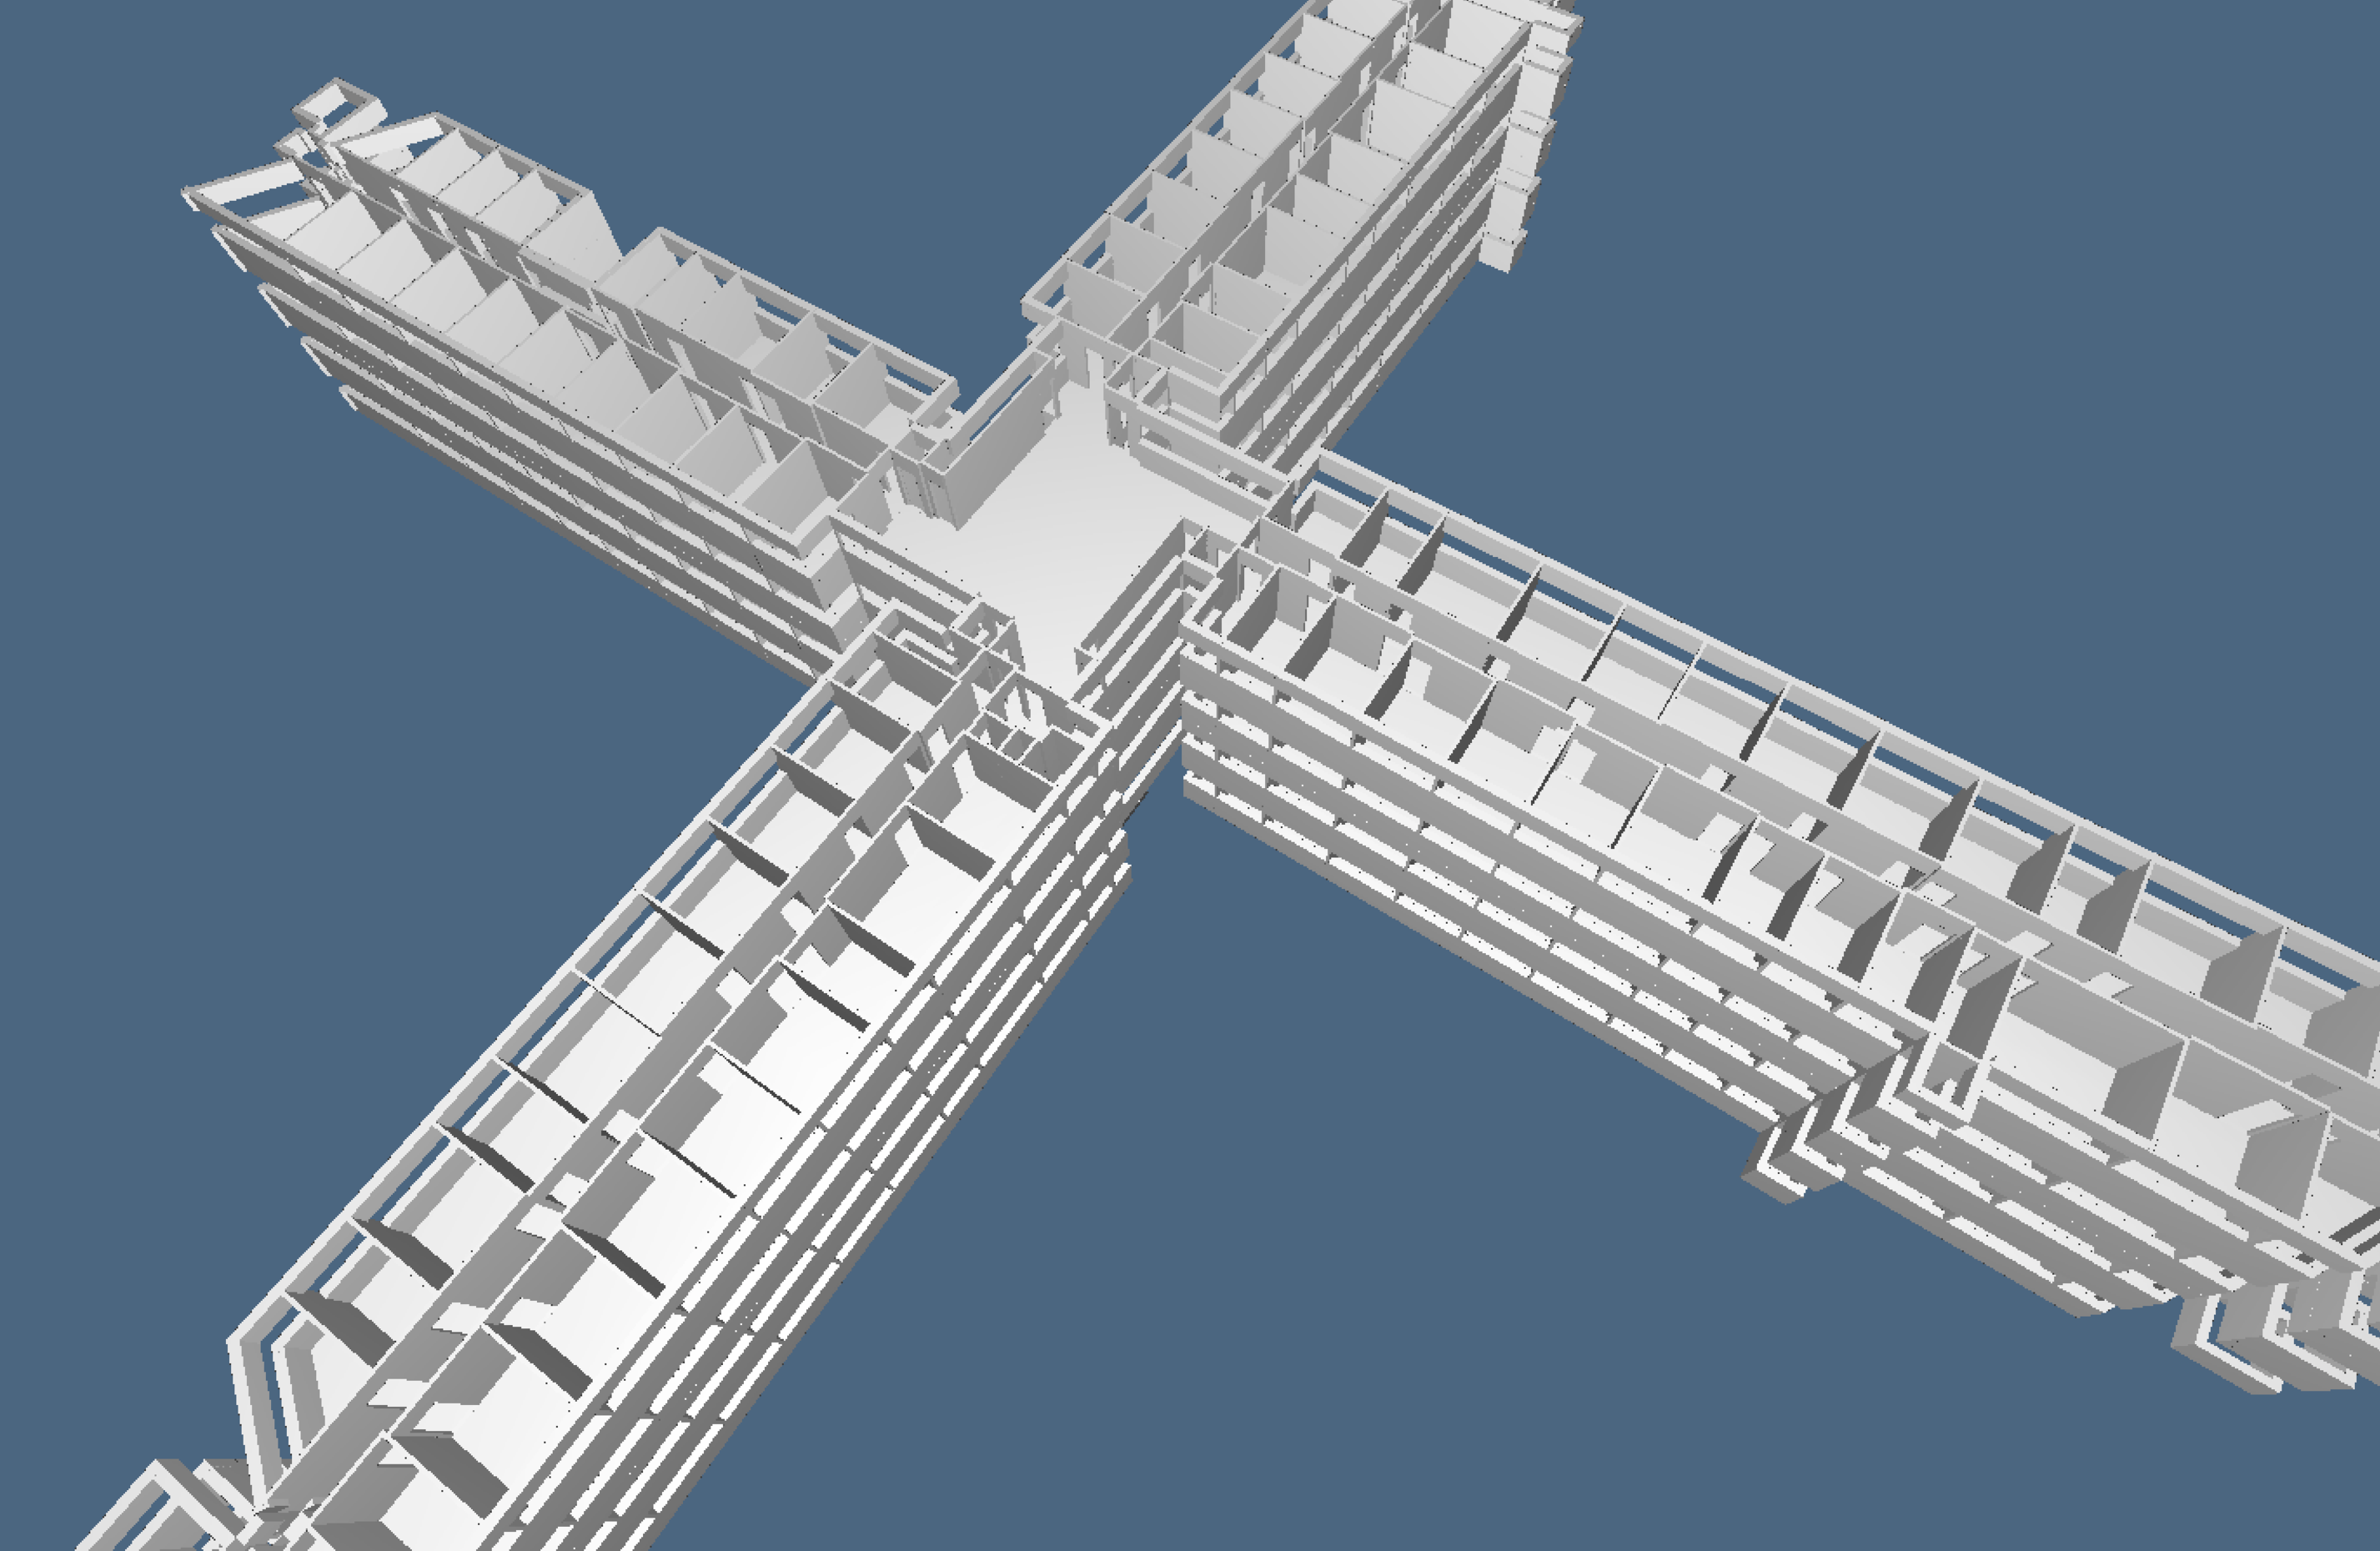
\includegraphics[width=0.325\linewidth]{images/tower1} 
   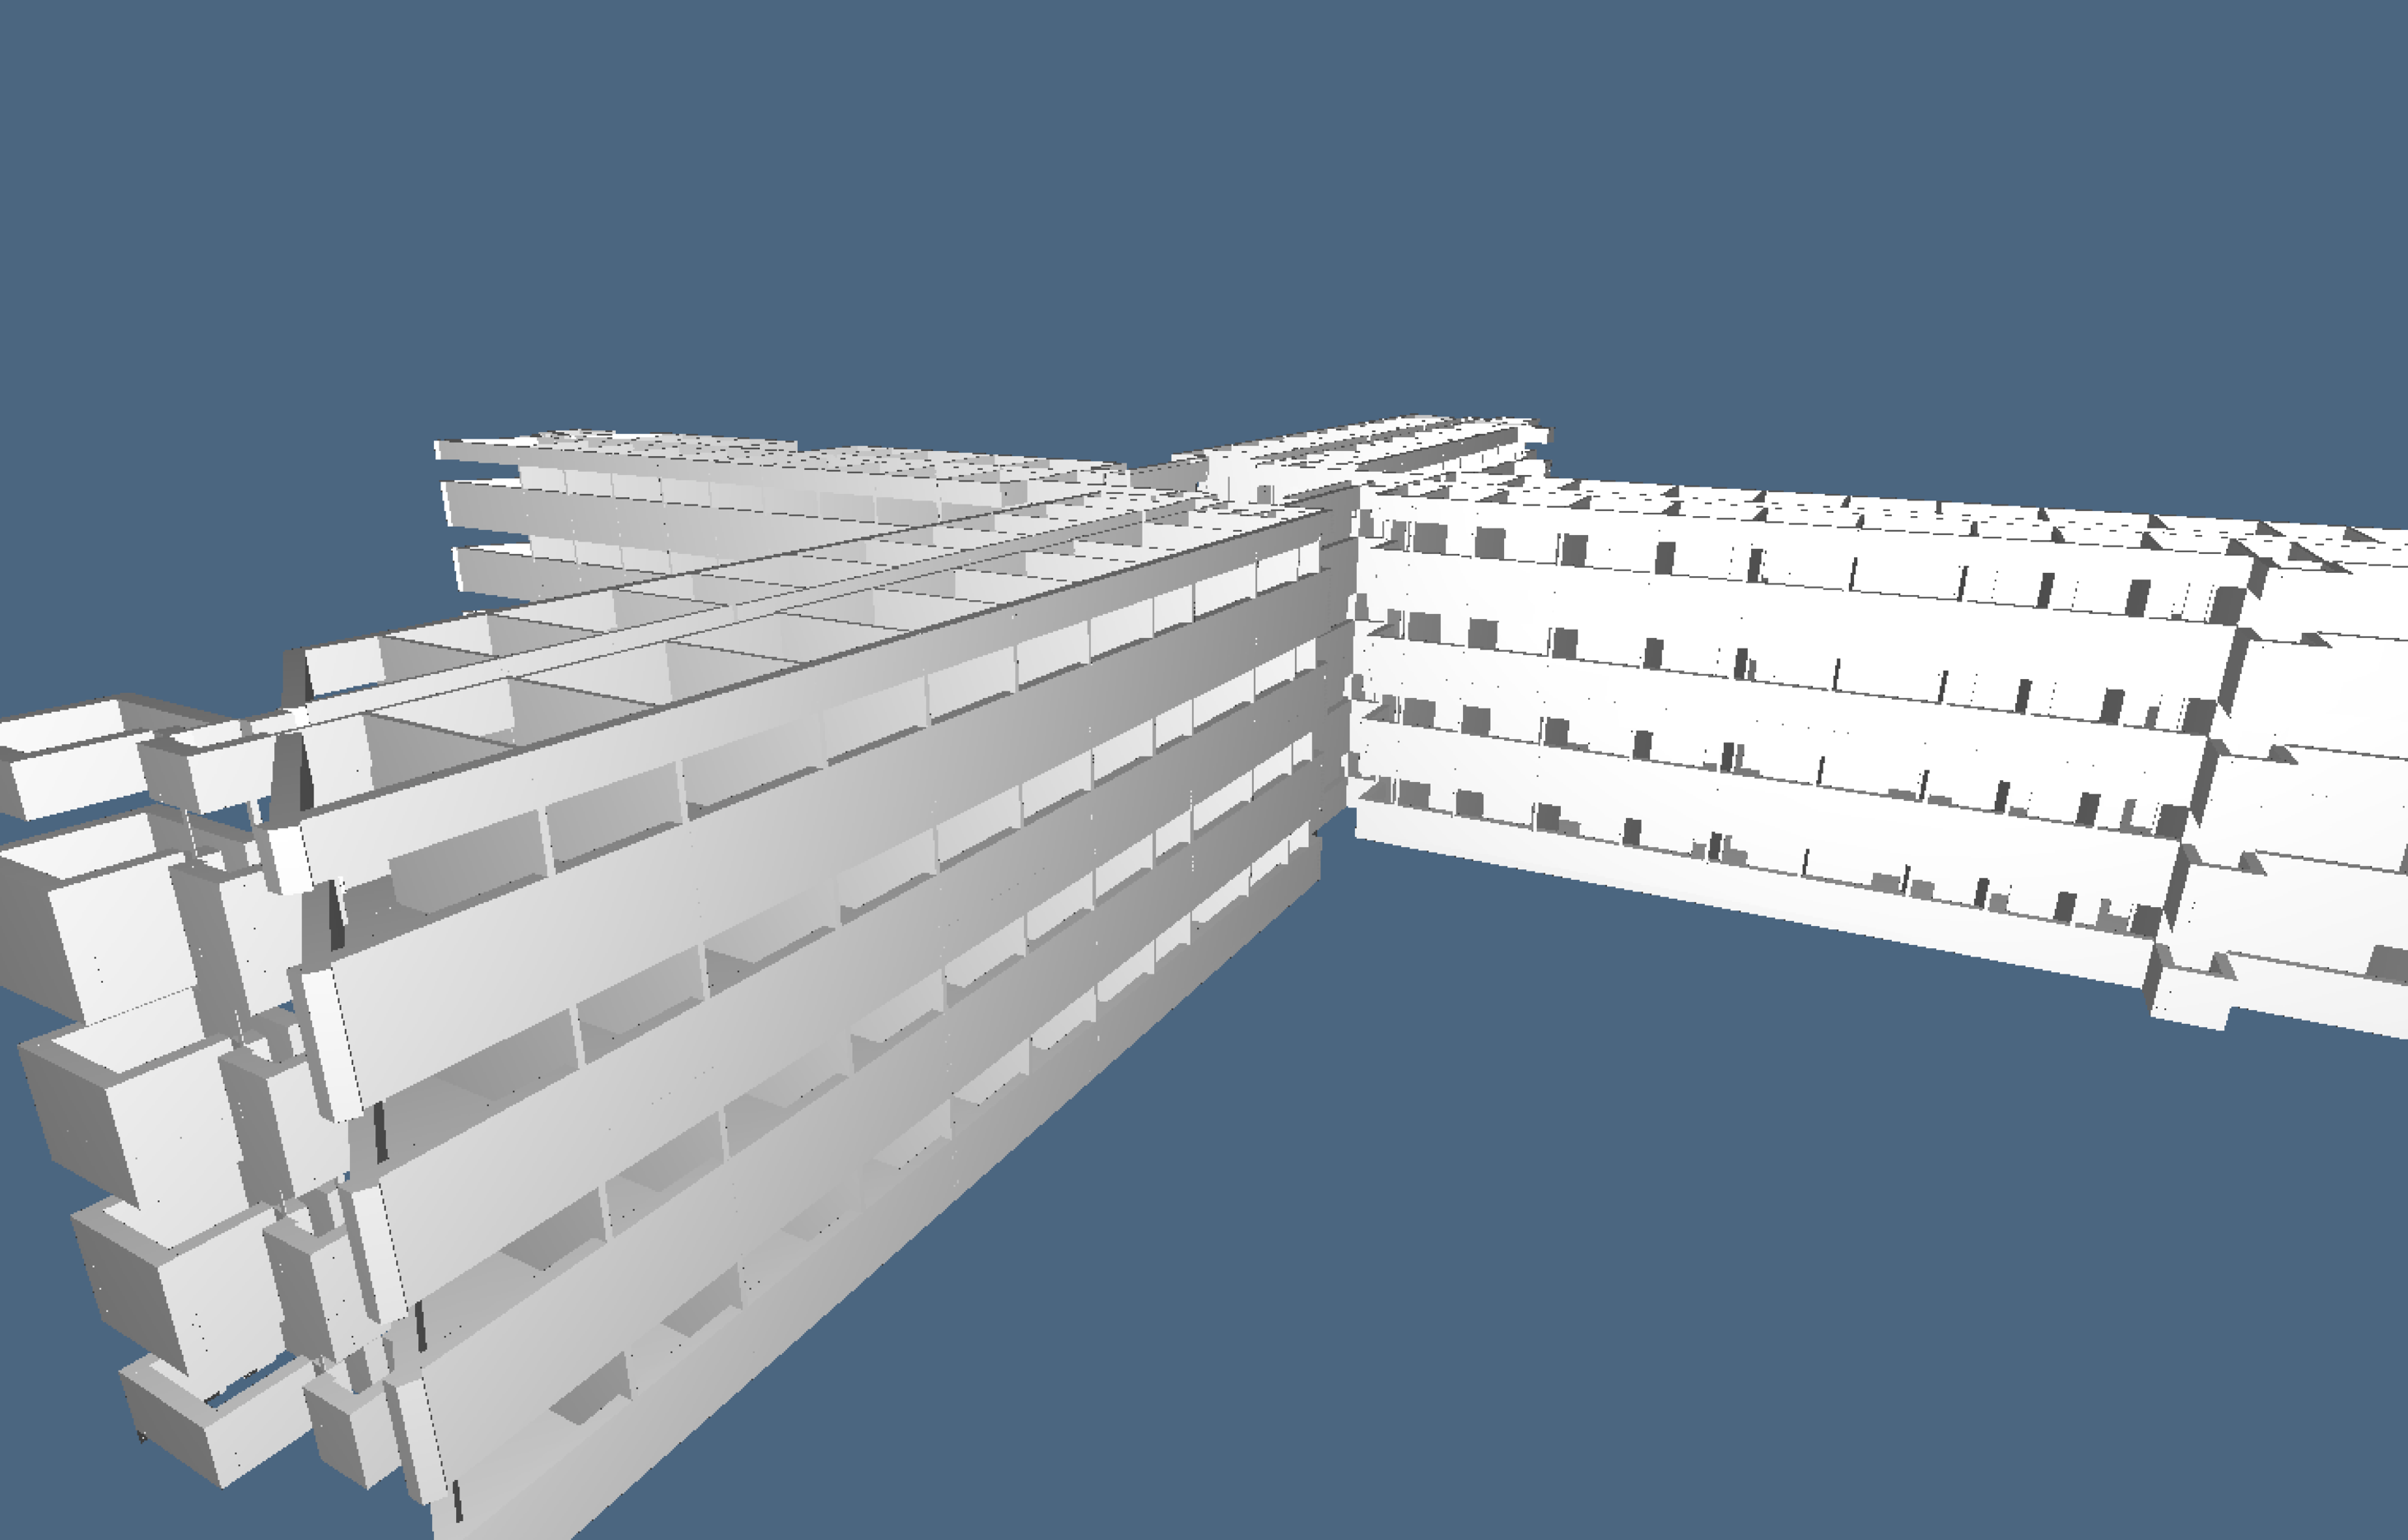
\includegraphics[width=0.325\linewidth]{images/tower2} 
   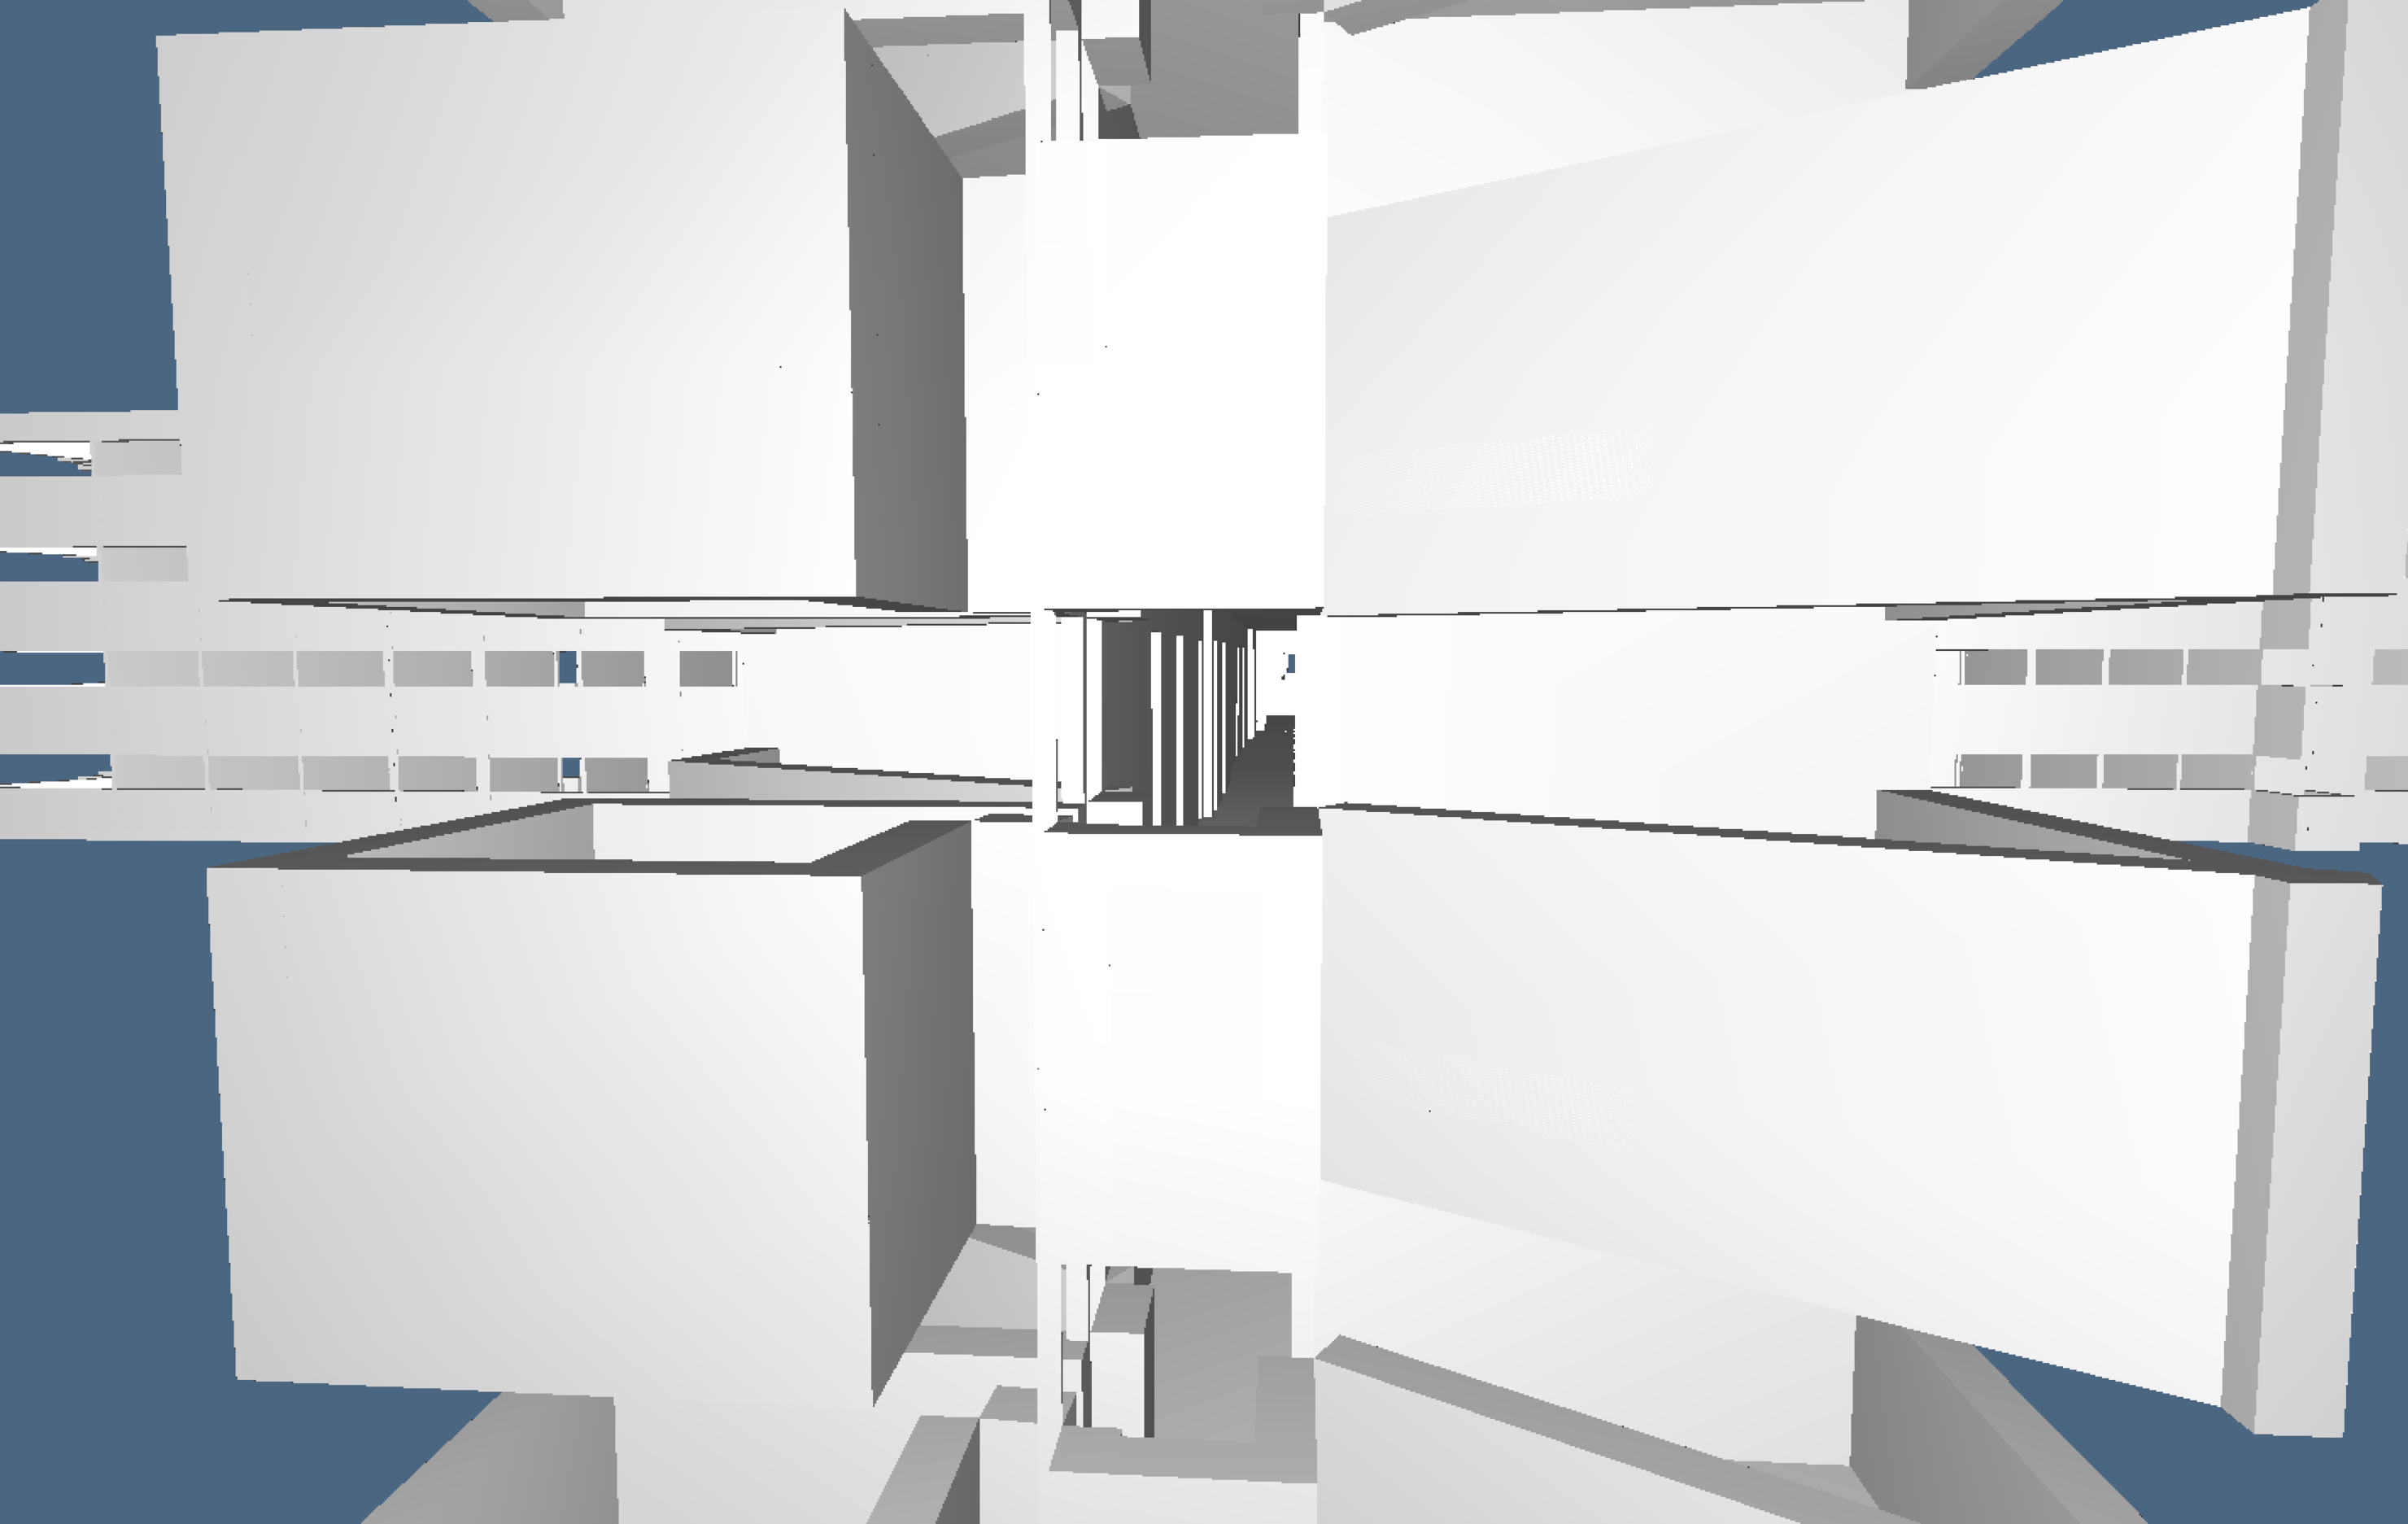
\includegraphics[width=0.325\linewidth]{images/tower3} 
   \caption{(a) Top view of the business tower building model; (b) exterior view; (c) close view.}
   \label{fig:towerplan1}
\end{figure}


%-------------------------------------------------------------------------------
\subsection{Exporting of test example}
%-------------------------------------------------------------------------------

\paragraph{Exporting of test example}
%-------------------------------------------------------------------------------
@O test/py/architectural/test06.py
@{""" Construction and visualization of a business tower building """

@< Input of floorplan wire-frame @>
@< Generation of 2-cellular complexes @>
@< Selection of specialized 1-chains @>
@< Guides: 1-chains embedded in 3D @>
@< 2.5D chains of the whole building @>
@< Construction of 3D floor slabs (pyplasm) @>
@< Assembly of 3D model @>
@< Visualization of whole tower building @>
@}
%-------------------------------------------------------------------------------


%-------------------------------------------------------------------------------
%===============================================================================
\section{The ABC computational framework}\label{sec:library}
%===============================================================================
%-------------------------------------------------------------------------------
\subsection{ABC: a set of classes}
%-------------------------------------------------------------------------------

We have already specified some geometric and topological conchps as a set of basic ABC classes: vertices and cells, models, structures and assemblies. Such basis classes are further specialized by a hierarchy of subclasses adding detailed semantics relative to the particular class of buildings under consideration and/or the considered construction technology and process.


%-------------------------------------------------------------------------------
\subsection{Some specialised methods}
%-------------------------------------------------------------------------------
2 column
%-------------------------------------------------------------------------------
\subsection{Zero install: working in the browser}
%-------------------------------------------------------------------------------
0.5 column
%-------------------------------------------------------------------------------

%-------------------------------------------------------------------------------
%===============================================================================
\section{Software module contents}\label{sec:library}
%===============================================================================
%-------------------------------------------------------------------------------
\subsection{From faces to list of edges}

Some transformations of 2D data are given In this section. 

\paragraph{From faces FV to list of edges EV}
The \texttt{face2edge} operator takes every consecutive pair of vertex indices from each face and return such list of pairs (i.e.~the \texttt{EV} relation), filtered from double instances.
%-------------------------------------------------------------------------------
@D From faces FV to list of edges EV
@{def face2edge(FV):
    """ From faces to list of edges """
    edges = AA(sorted)(CAT([TRANS([face, face[1:]+[face[0]]]) for face in FV]))
    return AA(eval)(set(AA(str)(edges)))
@}
%-------------------------------------------------------------------------------

\paragraph{From LAR model to list of polylines}
The function \texttt{lar2polylines}
transforms a LAR model into a list of polylines, i.e.~of (closed) lists of 2D points, where the last point coincides with the first one.
%-------------------------------------------------------------------------------
@D From faces FV to list of edges EV
@{def lar2polylines (model):
    """ From LAR model to list of polylines """
    V,FV = model
    return [[V[v] for v in cell]+[V[cell[0]]] for cell in FV]
@}
%-------------------------------------------------------------------------------

\paragraph{From LAR model to list of lines}
The function \texttt{lar2polylines}
transform a LAR model into a list of lines, i.e.~of pairs of points.
%-------------------------------------------------------------------------------
@D From faces FV to list of edges EV
@{def lar2lines (model):
    """ From LAR model to list of lines """
    V,EV = model
    return [[V[v] for v in cell] for cell in EV]
@}
%-------------------------------------------------------------------------------

\paragraph{Boundary cells ($2D\to 1D$) computation}
The computations of boundary cells is executed by calling the \texttt{boundaryCells} from the \texttt{larcc} module.

%-------------------------------------------------------------------------------
@D Boundary cells ($2D\to 1D$) computation
@{def lar2boundaryEdges(FV,EV):
    """ Boundary cells computation """
    return boundaryCells(FV,EV)
@}
%-------------------------------------------------------------------------------

\paragraph{Interior partitions ($2D\to 1D$) computation}
The indices of the boundary 1-cells are returned in \texttt{boundarychain1}, and subtracted from the set $\{0,1,\ldots,|E|-1\}$ in order to return the indices of the \texttt{interiorCells}.
%-------------------------------------------------------------------------------
@D Interior partitions ($2D\to 1D$) computation
@{def lar2InteriorEdges(FV,EV):
    """ Boundary cells computation """
    boundarychain1 = boundaryCells(FV,EV)
    totalChain1 = range(len(EV))
    interiorCells = set(totalChain1).difference(boundarychain1)
    return interiorCells
@}
%-------------------------------------------------------------------------------


\subsection{Geometric aggregation of building units}

Several methods can be used to to aggregate the LAR models \texttt{[V,CV]} and  \texttt{[W,CW]} of two building units into one single structure. The method provided by the \texttt{movePoint2point(twoModels)} function aggregates the vertices of two models after having applied a translation \texttt{t()} to the second set of vertices (\texttt{W}). The translation vector is computed as vector difference of \texttt{pointQ}
and \texttt{pointP}.

\paragraph{Move : $Model \times Model \to Model$ operator}
%-------------------------------------------------------------------------------
@D Move ($P\to Q$) operator
@{def movePoint2point(twoModels):
    """ Move (P -> Q) operator """
    def movePoint2point0(pointP):
        def movePoint2point1(pointQ):
            [V,CV], [W,CW] = twoModels
            mat = t( *DIFF([pointP,pointQ]) )
            [W,CW] = larApply(mat)([W,CW])
            print "\n W =",W
            print "\n CW =",CW
            n = len(V)
            return [ V+W, CV+[[w+n for w in REVERSE(cell)] for cell in CW] ] 
        return movePoint2point1    
    return movePoint2point0
@}
%-------------------------------------------------------------------------------


\paragraph{Parametric spiral stair}

A fully parametric \texttt{spiralStair} functions is given below, where the major and minor radiuses \texttt{R} and \texttt{r}, the step \texttt{riser}, the spiral \texttt{pitch}, i.e.~the distance between two turns, the real number of turns \texttt{nturns} and the number of \texttt{steps} for every $2\pi$ angle can be user-specified.

%-------------------------------------------------------------------------------
@D Trasform a solid helicoid into a spiral stair
@{def spiralStair(width=0.2,R=1.,r=0.5,riser=0.1,pitch=2.,nturns=2.,steps=18):
    V,CV = larSolidHelicoid(width,R,r,pitch,nturns,steps)()
    W = CAT([[V[k],V[k+1],V[k+2],V[k+3]]+
        [SUM([V[k+1],[0,0,-riser]]),SUM([V[k+3],[0,0,-riser]])]
        for k,v in enumerate(V[:-4]) if k%4==0])
    for k,w in enumerate(W[:-12]):
        if k%6==0: W[k+1][2] = W[k+10][2]; W[k+3][2] = W[k+11][2]
    nsteps = len(W)/12
    CW =[SUM([[0,1,2,3,6,8,10,11],[6*k]*8]) for k in range(nsteps)]
    return W,CW

if __name__=="__main__":
    VIEW(STRUCT(MKPOLS(spiralStair())))
    VIEW(SKEL_1(STRUCT(MKPOLS(spiralStair()))))
    VIEW(STRUCT(MKPOLS(spiralStair(0.1))))
@}
%-------------------------------------------------------------------------------

%-------------------------------------------------------------------------------
\subsection{Exporting the library}
%-------------------------------------------------------------------------------

@O larlib/larlib/architectural.py
@{""" architectural module """
@< Initial import of modules @>
@< From faces FV to list of edges EV @>
@< Some operators for assemblies @>
@< Low-dimensional constructors: 1D and 0D @>
@< Subdivide the 1-cells @>
@< Boundary cells ($2D\to 1D$) computation @>
@< Interior partitions ($2D\to 1D$) computation @>
@< Move ($P\to Q$) operator @>
@< Subdivide the 1-cells of the concept plan @>
@< Trasform a solid helicoid into a spiral stair @>
@< Specialized version of solidify operator for horizontal 3D polygons @>
@< Horizontal closures generator @>
@< Placing a 3D object (wall) with possible solid subtraction (door) @>
@}
%===============================================================================
\section{Conclusion}\label{sec:conclusion}
%===============================================================================
%-------------------------------------------------------------------------------
\subsection{The state of the art}
%-------------------------------------------------------------------------------
0.5 column
%-------------------------------------------------------------------------------
\subsection{What next}
%-------------------------------------------------------------------------------
0.5 column

\bibliographystyle{amsalpha}
\bibliography{architectural}
1.5 column
= 10 pages

%-------------------------------------------------------------------------------
%===============================================================================
\appendix
\section{Appendix}
\section{Utility functions}
%===============================================================================

\paragraph{Initial import of modules}

%-------------------------------------------------------------------------------
@D Initial import of modules
@{""" Initial import of modules """
from larlib import *
@}
%-------------------------------------------------------------------------------

\section{Tests}


\paragraph{Concept design}

%-------------------------------------------------------------------------------
@O test/py/architectural/test01.py
@{""" Concept design """
@< Initial import of modules @>
@< Input of LAR architectural plan @>
# VIEW(STRUCT(AA(POLYLINE)(lar2polylines (model))))
# VIEW(EXPLODE(1.2,1.2,1)(AA(POLYLINE)(lar2polylines (model))))
bU = AA(SOLIDIFY)(AA(POLYLINE)(lar2polylines (dwelling)))
# VIEW(EXPLODE(1.2,1.2,1)(bU))
EV = face2edge(FV)
VIEW(EXPLODE(1.2,1.2,1)(MKPOLS((V,EV))))

eE,iP = bUnit_to_eEiP(FV,EV)
modEe1D = V, [EV[e] for e in eE]
modIp1D = V, [EV[e] for e in iP]
eE1D = AA(COLOR(RED))(MKPOLS(modEe1D))
iP1D = AA(COLOR(GREEN))(MKPOLS(modIp1D))

VIEW(EXPLODE(1.2,1.2,1)(eE1D))
VIEW(EXPLODE(1.2,1.2,1)(iP1D))
VIEW(STRUCT(bU + iP1D + eE1D))
VIEW(EXPLODE(1.2,1.2,1)(bU + iP1D + eE1D))

floorHeight = larIntervals([1])([4])
modIp2D = larModelProduct([ modIp1D, floorHeight ])
modEe2D = larModelProduct([ modEe1D, floorHeight ])

VIEW(EXPLODE(1.2,1.2,1)(bU + MKPOLS(modIp2D) + eE1D))
VIEW(EXPLODE(1.2,1.2,1)(bU + iP1D + MKPOLS(modEe2D)))
VIEW(EXPLODE(1.2,1.2,1)(bU + MKPOLS(modIp2D) + MKPOLS(modEe2D)))
@}
%-------------------------------------------------------------------------------



%-------------------------------------------------------------------------------
@O test/py/architectural/test02.py
@{""" test file """
@< Initial import of modules @>
@< Input of LAR architectural plan @>
(W,FW) = larApply(s(-1,-1))(dwelling)
(V,FV) = dwelling
(V,FV) = movePoint2point([ (V,FV),(W,FW) ])(V[20])(W[25])
EV = face2edge(FV)
VIEW(EXPLODE(1.2,1.2,1)(MKPOLS((V,EV))))
@}
%-------------------------------------------------------------------------------



%-------------------------------------------------------------------------------
@D Specialized version of solidify operator for horizontal 3D polygons
@{""" Solidify horizontal polygons in 3D """
def solidify(pol):    
    min=MIN([1])(pol)[0]
    max=MAX([1])(pol)[0]
    z = MIN([3])(pol)[0]
    pol = PROJECT(1)(pol)
    siz=max-min
    far_point=max+siz*100 
    def InftyProject(pol):
        verts,cells,pols=UKPOL(pol)
        verts=[[far_point] + v[1:] for v in verts]
        return MKPOL([verts,cells,pols])  
    ret=SPLITCELLS(pol)
    ret=[JOIN([pol,InftyProject(pol)]) for pol in ret]
    return T(3)(z)(XOR(ret))
@}
%-------------------------------------------------------------------------------

\paragraph{Placing a 3D object (wall) with possible solid subtraction (door)}
%-------------------------------------------------------------------------------
@D Placing a 3D object (wall) with possible solid subtraction (door)
@{""" Placing a 3D object (wall) with possible solid subtraction (door) """

def place(obj):

    def dist(p1,p2):
        return SQRT(SQR(p1[0]-p2[0])+SQR(p1[1]-p2[1]))

    depth,length,height = SIZE([1,2,3])(obj)
    p = array(MIN([1,2,3])(obj))
    obj = T([1,2,3])(list(-1*p))(obj)
    obj = S(2)(1./length)(obj)
    def place0(obj2=None):
        def place01(line):
            x,y,z = VECTDIFF([line[1],line[0]])
            angle = -math.atan2(x,y)
            outObj = S(2)(dist(line[1],line[0]))(obj)
            if isinstance(obj2,pyplasm.xgepy.Hpc):
                outObj = DIFFERENCE([outObj,obj2])
            outObj = R([1,2])(angle)(outObj)
            outObj = T([1,2,3])(line[0])(outObj)
            return outObj
        return place01
    return place0
@}
%-------------------------------------------------------------------------------


\end{document}
